% !TEX TS-program = latexmk
% !TEX encoding = UTF-8 Unicode

% This is a book in LaTeX 2e. 
% To compile the file, you need to use the following command line commands in Linux:
%	pdflatex --shell-escape -synctex=1  -recorder metric-space-notes.tex
%	bibtex metric-space-notes 
%	makeindex -s notation.gst -o not.gls not.glo  
%	makeindex metric-space-notes
% and repeat each of these many times.
\documentclass{willowtreebook}

\Title{Notes on Metric Spaces}
\Author{\texorpdfstring{Benjamin \scotsMc{}Kay}{Benjamin McKay}}
%\Location{University College Cork}
%\BibliographyFile{metric-space-notes}
\usepackage{standalone}
\DeclareFontFamily{OMX}{lmex}{}
\DeclareFontShape{OMX}{lmex}{m}{n}{<-> lmex10}{}

\DeclareUnicodeCharacter{2227}{\ensuremath{\wedge}}
\DeclareUnicodeCharacter{2207}{\ensuremath{\nabla}} %∇
\DeclareUnicodeCharacter{00A3}{\ensuremath{\LieDer}} %£
\DeclareUnicodeCharacter{02E9}{\ensuremath{\hook}} %˩
\DeclareUnicodeCharacter{2308}{\ensuremath{\lceil}}
\DeclareUnicodeCharacter{2309}{\ensuremath{\rceil}}
\DeclareUnicodeCharacter{230A}{\ensuremath{\lfloor}}
\DeclareUnicodeCharacter{230B}{\ensuremath{\rfloor}}
\DeclareUnicodeCharacter{03F5}{\ensuremath{\varepsilon}}
\DeclareUnicodeCharacter{2282}{\ensuremath{\subset}}%⊂
\DeclareUnicodeCharacter{03C6}{\ensuremath{\phi}}%ϕ
\DeclareUnicodeCharacter{03D5}{\ensuremath{\varphi}}%ϕ
\DeclareUnicodeCharacter{2297}{\otimes}
\DeclareUnicodeCharacter{03C9}{\ensuremath{\omega}}%
\DeclareUnicodeCharacter{222B}{\int}%
\DeclareUnicodeCharacter{221E}{\infty}%
\DeclareUnicodeCharacter{2211}{\sum}%
\DeclareUnicodeCharacter{03B1}{\alpha}%
\DeclareUnicodeCharacter{03B2}{\beta}%
\newunicodechar{ℝ}{\mathbb{R}}
\newunicodechar{ϕ}{\varphi}
\newunicodechar{⟨}{\left<}
\newunicodechar{⟩}{\right>}

\NewDocumentCommand\textprime{}{\ensuremath{'}}

%\usepackage{tensor}% for upper and lower indices
%
%\usepackage{mathrsfs}%the \mathscr command for script fonts
%
%\usepackage{mleftright}% fixes problems with \left and \right
%
%\usepackage{verbatim}
%% For verbatim quotation of programming code.
%
%\usepackage{siunitx}

% TiKZ graphics packages
\usepackage{brunnian}
\usepackage{tikz}
\usetikzlibrary{%
matrix,%
arrows,%
arrows.meta,%
calc,%
decorations.pathmorphing,%
decorations.pathreplacing,%
decorations.markings,%
decorations.fractals,%
fadings,%
hobby,%
knots,%
shadows,%
lindenmayersystems,%
shadings,%
backgrounds,%
angles,%
quotes}
\usepackage{pgfplots}
\usepgfplotslibrary{polar}
\usepgfplotslibrary{fillbetween}
\usepackage{tikz-3dplot}
%\usepackage{tkz-graph}
\usepackage{tikz-cd}
\usepackage{tqft}
\usepackage{cprotect}
\usepackage{colortbl}

% We don't need to worry about the pdf page groups, so we ignore these warnings.
\pdfsuppresswarningpagegroup=1

%%.....Mathematics Commands
\def\cprime{\('\)} % For Russian names

% for definitions, A \defeq B means A is defined to be B.
\newcommand*{\defeq}{\mathrel{\vcenter{\baselineskip0.5ex \lineskiplimit0pt
                     \hbox{\scriptsize.}\hbox{\scriptsize.}}}%
                     =}


% I don't like the default \Re and \Im 
% for complex numbers.
\renewcommand{\Re}{\ensuremath{\operatorname{Re}}}
\renewcommand{\Im}{\ensuremath{\operatorname{Im}}}

% Various sets
\newcommand*{\Z}[1]{\ensuremath{\mathbb{Z}^{#1}}}
\newcommand*{\R}[1]{\ensuremath{\mathbb{R}^{#1}}}
\newcommand*{\Q}[1]{\ensuremath{\mathbb{Q}^{#1}}}
\newcommand*{\C}[1]{\ensuremath{\mathbb{C}^{#1}}}
\newcommand*{\Quat}[1]{\ensuremath{\mathbb{H}^{#1}}}

% Brackets
\newcommand*{\pr}[1]{\ensuremath{\left(#1\right)}}
\newcommand*{\curly}[1]{\ensuremath{\left\{#1\right\}}}
\newcommand*{\of}[1]{\ensuremath{\pr{#1}}}

% Matrices
\newcommand*{\matrixExtraVerticalSpace}{1.2}
\makeatletter
\renewcommand*\env@matrix[1][\arraystretch]{%
  \edef\arraystretch{#1}%
  \hskip -\arraycolsep
  \let\@ifnextchar\new@ifnextchar
  \array{*\c@MaxMatrixCols c}}
\makeatother

% Vectors
\newcommand*\vectr[1]%
{%%
\begin{pmatrix}#1{}\end{pmatrix}
}%%

% ball
\NewDocumentCommand\ball{somm}%[metric space]{radius}{center}
{%
\IfValueTF{#2}%
{B_{#3}\of{#4,#2}}%
{%% else
\IfBooleanTF{#1}%
{B_{#3}\of{#4}}%
{B_{#3}#4}%
}%%
}%

% closed ball
\NewDocumentCommand\ballClosed{somm}%[metric space]{radius}{center}
{%
\IfValueTF{#2}%
{\bar{B}_{#3}\of{#4,#2}}%
{%% else
\IfBooleanTF{#1}%
{\bar{B}_{#3}\of{#4}}%
{\bar{B}_{#3}#4}%
}%%
}%

% Open subset of
\NewDocumentCommand\op{m}{\text{open } \subset #1}

% little o
\newcommand*{\littleo}[1]{\ensuremath{o\of{#1}}}

% volume:
% \vol{X} for Vol X, \vol*{X} for Vol(X).
\NewDocumentCommand\vol{sm}%
{%
\IfBooleanTF{#1}%
{\ensuremath{\operatorname{Vol}\of{#2}}}%
{\ensuremath{\operatorname{Vol}#2}}%
}%

% area
\NewDocumentCommand\area{sm}%
{%
\IfBooleanTF{#1}%
{\ensuremath{\operatorname{Area}\of{#2}}}%
{\ensuremath{\operatorname{Area}#2}}%
}%

% length
\NewDocumentCommand\length{sm}%
{%
\IfBooleanTF{#1}%
{\ensuremath{\operatorname{length}\of{#2}}}%
{\ensuremath{\operatorname{length}#2}}
}%

\NewDocumentCommand\conv{mm}%
{%
#1*#2%
}%


% Transpose
\newcommand*{\trans}[1]{{#1}^t}

% Inner product 
\newcommand*{\ip}[2]{\ensuremath{\left<#1,#2\right>}}

% Inner product 
\NewDocumentCommand\Span{om}{\ensuremath{\IfValueTF{#1}{\left<#1\right>_{#2}}{\left<#2\right>}}}

% Partial derivative
\newcommand*{\pd}[2]{\ensuremath{\frac{\partial #1}{\partial #2}}}

% Number of integer points
\NewDocumentCommand\intsin{sm}%
{%
\IfBooleanTF{#1}%
{\tensor[^{\#}]{(#2)}{}}%
{\tensor[^{\#}]{{#2}}{}}%
}%

% Hook
\NewDocumentCommand\hook{}{\ensuremath{\mathbin{\hbox{\vrule height1.4pt width4pt depth-1pt \vrule height4pt width0.4pt depth-1pt}}}}

% Lie derivative
\NewDocumentCommand\LieDer{}{\ensuremath{\EuScript L}}

% Adjoint
%\NewDocumentCommand\ad{m}{\ensuremath{#1^*}}
\DeclareMathOperator{\Kernel}{ker}
\DeclareMathOperator{\Image}{im}
\DeclareMathOperator{\rank}{rank}
\DeclareMathOperator{\tr}{tr} % trace
\DeclareMathOperator{\Pf}{Pf} % Pfaffian

\NewDocumentCommand\coface{om}{T^+_{\IfValueT{#1}{#1}{}}{#2}}
\NewDocumentCommand\conormal{om}{T^{\perp}_{\IfValueT{#1}{#1}{}}{#2}}
\NewDocumentCommand\cofac{om}{{#2}^+_{\IfValueT{#1}{#1}{}}}
\NewDocumentCommand\conorm{om}{{#2}^{\perp}_{\IfValueT{#1}{#1}{}}}

\NewDocumentCommand\cofacequo{om}{T^-_{\IfValueT{#1}{#1}{}}{#2}}
\NewDocumentCommand\cofacquo{om}{{#2}^-_{\IfValueT{#1}{#1}{}}}


% Classical groups
\NewDocumentCommand\Gp{mm}{\ensuremath{\textrm{#1}\of{#2}}}
\NewDocumentCommand\GL{m}{\Gp{GL}{#1}}
\NewDocumentCommand\SL{m}{\Gp{SL}{#1}}
\NewDocumentCommand\PSL{m}{\mathbb{P}\Gp{SL}{#1}}
\NewDocumentCommand\PGL{m}{\mathbb{P}\Gp{GL}{#1}}
\NewDocumentCommand\SO{m}{\Gp{SO}{#1}}
\NewDocumentCommand\Orth{m}{\Gp{O}{#1}}
\NewDocumentCommand\Un{m}{\Gp{U}{#1}}
\NewDocumentCommand\Symp{m}{\Gp{Sp}{#1}}
\NewDocumentCommand\Or{m}{\operatorname{O}\left({#1}\right)}
\NewDocumentCommand\SOp{m}{\operatorname{SO}^{+}\left({#1}\right)}
\NewDocumentCommand\PO{m}{\operatorname{\mathbb{P}O}\left({#1}\right)}
\NewDocumentCommand\LieSO{m}{\LieAlgebra{SO}{#1}}
\newcommand{\LieGL}[1]{\mathfrak{gl}\left({#1}\right)}
\newcommand{\LieSL}[1]{\mathfrak{sl}\left({#1}\right)}
\newcommand{\LieOr}[1]{\mathfrak{o}\left({#1}\right)}
\newcommand{\LieSymp}[1]{\mathfrak{sp}\left({#1}\right)}
\newcommand{\PSymp}[1]{\operatorname{\mathbb{P}Sp}\left({#1}\right)}
\newcommand{\SU}[1]{\operatorname{SU}\left({#1}\right)}
\newcommand{\LieSU}[1]{\mathfrak{su}\left({#1}\right)}
\newcommand{\PSU}[1]{\operatorname{\mathbb{P}SU}\left({#1}\right)}
\newcommand{\LieUn}[1]{\mathfrak{u}\left({#1}\right)}
\newcommand{\PUn}[1]{\operatorname{\mathbb{P}U}\left({#1}\right)}
\NewDocumentCommand\Ad{om}{\IfValueTF{#1}{\operatorname{Ad}_{#1}#2}{\operatorname{Ad}#2}}
\NewDocumentCommand\ad{om}{\IfValueTF{#1}{\operatorname{ad}_{#1}#2}{\operatorname{ad}#2}}

\NewDocumentCommand\LieAlgebra{mm}{\ensuremath{\mathfrak{\MakeLowercase{#1}}\of{#2}}}
\newcommand{\LieG}{\mathfrak{g}}
\newcommand{\LieH}{\mathfrak{h}}

\NewDocumentCommand\solvrad{m}{\sqrt{#1}}
\NewDocumentCommand\Levi{m}{{#1}^{\text{ss}}}

\NewDocumentCommand\CC{m}{\ensuremath{{#1}_{\C{}}}}


% Matrix norm
\NewDocumentCommand\norm{m}{\left\|#1\right\|}

%%%%
%%%% Graphics
%%%%

\newcommand*{\TwoDPlotColourOne}{blue!50}
\newcommand*{\TwoDPlotColourTwo}{olive!50!blue}
\newcommand*{\TwoDPlotColourThree}{olive!75!blue}
\newcommand*{\TwoDPlotColourFour}{olive!50}


% Miffy: drawing a little face.
\tikzstyle _grid=[gray!10,thin]
\NewDocumentCommand\miffy{}
{%
\filldraw[drop shadow, rounded corners,fill=brown!20,draw=brown] (-.6,-.6) rectangle (.6,.6); % background
    \draw (0,0) circle (.5); % boundary of face
    \fill (-0.05555cm,0) circle (.03cm); % left eye
    \fill (+.388889cm,0.05555cm) circle (.03cm); % right eye
    \draw (+.1666cm,-.1666cm) -- +(.103cm,-.0407cm);
    \draw (+.1666cm,-.21444cm) -- +(+.111cm,.0444cm);
}%
\NewDocumentCommand\gridInsideMiffysFace{}
% A grid to lie inside Miffy's face, so that
% we can make area comparisons.
{%
    \begin{scope}
    \draw[clip] (0,0) circle (.5); % boundary of face
    \draw[step=0.1,_grid] (-1,-1) grid (1,1);
    \end{scope}
}%
\NewDocumentCommand\nullMiffy{mmmm}%{a}{b}{c}{d}
% Matrix
% (a b)
% (c d)
{%
\draw%
(-.5cm*{sqrt(#1*#1+#2*#2)},-.5cm*{sqrt(#3*#3+#4*#4)})%
 --
(.5cm*{sqrt(#1*#1+#2*#2)},.5cm*{sqrt(#3*#3+#4*#4)});
}%
\NewDocumentCommand\distortedMiffy{mmmm}%{a}{b}{c}{d}
% Matrix
% (a b)
% (c d)
{%
\begin{scope}[cm={{#1},{#2},{#3},{#4},(0,0)}]%
\miffy%
\end{scope}
}%
\NewDocumentCommand\gridBehindMiffy{mmmm}%{a}{b}{c}{d}
% A grid to be drawn behind miffy,
% where miffy is distorted by the matrix
% (a b)
% (c d)
{%
    \draw[_grid,step=.5cm]
    (-.5cm*{ceil(sqrt({#1}*{#1}+{#2}*{#2}))},-.5cm*{ceil(sqrt({#3}*{#3}+{#4}*{#4}))})
    grid
    (.5cm*{ceil(sqrt({#1}*{#1}+{#2}*{#2}))},.5cm*{ceil(sqrt({#3}*{#3}+{#4}*{#4}))}) ;
}%


\tikzfading[name=fade left,
left color=transparent!70,
right color=transparent!0]

% mid-point rule
\pgfplotsset{
	compat=1.9,
    midpoint segments/.code={\pgfmathsetmacro\midpointsegments{#1}},
    midpoint segments=3,
    midpoint/.style args={#1:#2}{
        ybar interval,
        domain=#1+((#2-#1)/\midpointsegments)/2:#2+((#2-#1)/\midpointsegments)/2,
        samples=\midpointsegments+1,
        x filter/.code=\pgfmathparse{\pgfmathresult-((#2-#1)/\midpointsegments)/2}
    }
}


% right hand sums
\pgfplotsset{
    right segments/.code={\pgfmathsetmacro\rightsegments{#1}},
    right segments=3,
    right/.style args={#1:#2}{
        ybar interval,
        domain=#1+((#2-#1)/\rightsegments):#2+((#2-#1)/\rightsegments),
        samples=\rightsegments+1,
        x filter/.code=\pgfmathparse{\pgfmathresult-((#2-#1)/\rightsegments)}
    }
}

% left hand sums
\pgfplotsset{
    left segments/.code={\pgfmathsetmacro\leftsegments{#1}},
    left segments=3,
    left/.style args={#1:#2}{
        ybar interval,
        domain=#1:#2,
        samples=\leftsegments+1,
        x filter/.code=\pgfmathparse{\pgfmathresult}
       }
}



% Draw a vector field in the plane.

\newwrite\tempfile

\newcounter{vectorfieldcounter}
\setcounter{vectorfieldcounter}{0}


\newcommand*{\vectorfieldplot}[4]%%%
%% \vectorfield{2*x}{1+y}{2x}{1+y}
%% draws the vector field (2x,1+y) over -1 < x < 1, -1 < y < 1, with a title.
%% \vectorfield{2*x}{1+y}{}{}
%% draws the vector field (2x,1+y) over -1 < x < 1, -1 < y < 1, with no title.
{%%%%
\stepcounter{vectorfieldcounter}%
\IfFileExists{XXX\thevectorfieldcounter.pdf}%%
{%%
\def\empt{}
\def\temp{#3}
\ifx\temp\empt%%
\begin{tabular}{c}%%
\includegraphics[width=2cm]{XXX\thevectorfieldcounter.pdf}%%
\end{tabular}
\else%%
\begin{tabular}{c}%%
\((#3,#4)\) \\{}%% 
\includegraphics[width=2cm]{XXX\thevectorfieldcounter.pdf}%% 
\end{tabular}\fi
}%%
{\immediate\openout\tempfile=XXX\thevectorfieldcounter.asy%
\immediate\write\tempfile{settings.outformat="pdf";
settings.prc=false;
settings.render=16;
import graph;
pen vectorfieldcolour=.3*blue+.6*white+.1*black+.3bp;
size(2cm,0);
pair a=(-1,-1);
pair b=(1,1);
path vector(pair z) 
{
	real x=z.x;
	real y=z.y;
	return (0,0)--(#1,#2);
}
add(vectorfield(vector,a,b,10,vectorfieldcolour,arrow=Arrow(2.5pt)));
clip(box(a,b));}
\immediate\closeout\tempfile%
\immediate\write18{asy XXX\thevectorfieldcounter.asy}%
}%
}%%%%




% drawing a cut-away sphere:
\def\k{0.55191496}

\tikzset{
    sphere color/.store in=\spherecolor,
    sphere scale/.store in=\spherescale,
    sphere color=blue,
    sphere scale=1,
    sphere/.style={
        ultra thick,
        line join=round,
        draw=#1!75!black,
        ball color=#1,
    },
    sphere inside/.style={
        shading angle=180,
        sphere=#1!25!gray!75!black
    }
}

\newenvironment{sphere}[1][]
    {
        \begin{scope}[x=(0:1cm), y=(90:1cm), z=(260:0.25cm), #1]
            \path [sphere inside=\spherecolor, scale=\spherescale] 
            circle [radius=1];
    }
    {
        \path let \n1={cos 10}, \n2={sin 10} in [sphere=\spherecolor, scale=\spherescale, even odd rule, opacity=0.5]
        circle [radius=1] 
        % Rotate 10 degrees around the y and x axes
        [x={(\n1, \n2^2, \n2*\n1)},
         y={(0, \n1, \n2)}, 
         z={(-\n2, -\n1*\n2, \n1^2)}] (0,1,0) 
                .. controls ++( 0, 0,\k) and ++(0,\k, 0) .. (0, 0, 1)
                .. controls ++(\k, 0, 0) and ++(0, 0,\k) .. (1, 0, 0) 
                .. controls ++(0, \k, 0) and ++(\k,0, 0) .. (0, 1, 0);
        \end{scope}
    }

% For the coffee cup in the manifolds chapter.
\tikzfading[name=fade out, inner color=transparent!0, outer color=transparent!100]

\newcommand*{\linearApproxBox}[6]%
{%
\draw[thick,white,opacity=.5]
({#1-#3-#5},{#2-#4-#6}) --
({#1+#3-#5},{#2+#4-#6}) --
({#1+#3+#5},{#2+#4+#6}) --
({#1-#3+#5},{#2-#4+#6}) --
cycle;
}%

\NewDocumentCommand\contMaps{O{}mO{\R{}}}{\ensuremath{C^{#1}({#2},{#3})}}
\NewDocumentCommand\smoothMaps{mO{\R{}}}{\contMaps[\infty]{#1}[#2]}


\newcommand*{\pickcolor}[2]{\definecolor{currentcolor}{rgb}{#1,.5,#2}}
\newcommand*{\nForms}[2]{\ensuremath{\Omega^{#1}\of{#2}}}
\newcommand*{\topForms}[1]{\nForms{\operatorname{top}}{#1}}
\newcommand*{\coboundaries}[2]{\ensuremath{B^{#1}\of{#2}}}
\newcommand*{\cocycles}[2]{\ensuremath{Z^{#1}\of{#2}}}
\newcommand*{\cohomology}[2]{\ensuremath{H^{#1}\of{#2}}}
\newcommand*{\deRhamcohomology}[2]{\ensuremath{H_{\text{dR}}^{#1}\of{#2}}}
\newcommand*{\compactcohomology}[2]{\ensuremath{H_c^{#1}\of{#2}}}
\newcommand*{\boundaries}[2]{\ensuremath{B_{#1}\of{#2}}}
\newcommand*{\cycles}[2]{\ensuremath{Z_{#1}\of{#2}}}
\NewDocumentCommand\homology{O{}mm}{\ensuremath{H^{#1}_{#2}\of{#3}}}
\NewDocumentCommand\BMhomology{mm}{\ensuremath{H^{\text{BM}}_{#1}\of{#2}}}
%\newcommand*{\homology}[2]{\ensuremath{H_{#1}\of{#2}}}
\usepackage{xspace}
\newcommand*{\Cech}{\v{C}ech\xspace}
\newcommand*{\CD}{\Cech--de~Rham\xspace}
\newcommand*{\CDchains}[2]{\ensuremath{\check\Omega^{#1}\of{#2}}}
\newcommand*{\CDcoboundaries}[2]{\ensuremath{\check{B}^{#1}\of{#2}}}
\newcommand*{\CDcocycles}[2]{\ensuremath{\check{Z}^{#1}\of{#2}}}
\newcommand*{\CDcohomology}[2]{\ensuremath{\check{H}^{#1}\of{#2}}}
\newcommand*{\CDd}{d}
\newcommand*{\topcohomology}[1]{\cohomology{\operatorname{top}}{#1}}
\newcommand*{\topcompactcohomology}[1]{\compactcohomology{\operatorname{top}}{#1}}
\newcommand*{\relativecohomology}[3]{\ensuremath{H^{#1}\of{#2;#3}}}
\newcommand*{\testforms}[2]{\ensuremath{\mathscr{D}^{#1}\of{#2}}}
\newcommand*{\allforms}[2]{\ensuremath{\mathscr{E}^{#1}\of{#2}}}
\newcommand*{\currentsdim}[2]{\ensuremath{\mathscr{D}'{}^{#1}\of{#2}}}
\newcommand*{\currentsdeg}[2]{\ensuremath{\mathscr{D}'_{#1}\of{#2}}}
\newcommand*{\supp}[1]{\ensuremath{\operatorname{supp} #1}}
\newcommand*{\Cnorm}[2]{\ensuremath{\norm{#2}_{C^{#1}}}}
\NewDocumentCommand\Cont{mm}{\ensuremath{C^{#1}\of{#2}}}
\NewDocumentCommand\Smooth{m}{\ensuremath{\Cont{\infty}{#1}}}
\newcommand{{\bull}}{{\scriptscriptstyle{\bullet}}}
\newcommand*{\complex}[1]{\ensuremath{#1^\bull}}
\newcommand*{\flag}[1]{\ensuremath{#1_\bull}}
\newcommand*{\flagvariety}[1]{\ensuremath{\operatorname{Fl}_{#1}}}
\newcommand*{\partialflagvariety}[2]{\ensuremath{\operatorname{Fl}^{#1}_{#2}}}
\newcommand*{\cohomologycomplex}[1]{\ensuremath{\cohomology{\bull}{#1}}}
\newcommand*{\Proj}[1]{\ensuremath{\mathbb{P}{#1}}}
\NewDocumentCommand\ProjCot{O{}m}{\ensuremath{\mathbb{P}T_{#1}^*#2}}
%\NewDocumentCommand\CotRay{O{}m}{\ensuremath{ST^*_{#1}#2}}
\newcommand*{\Gr}[2]{\ensuremath{\operatorname{Gr}_{#1}\!{#2}}}
\newcommand*{\gr}[1]{\ensuremath{\operatorname{gr} #1}}
\newcommand*{\id}{\ensuremath{\operatorname{id}}}
\newcommand*{\Div}[1]{\ensuremath{\operatorname{div}\of{#1}}}
\newcommand*{\graph}[1]{\ensuremath{\operatorname{graph}\of{#1}}}
% Principal value integral
\newcommand*{\pv}{\mathop{\mathrm PV}\!}
\newcommand*{\RP}[1]{\ensuremath{\mathbb{RP}^{#1}}}
\newcommand*{\CP}[1]{\ensuremath{\mathbb{CP}^{#1}}}
\newcommand*{\HP}[1]{\ensuremath{\mathbb{HP}^{#1}}}
\newcommand*{\Sym}[2]{\ensuremath{\operatorname{Sym}^{#1}\of{#2}}}
\NewDocumentCommand\Lm{smm}{\IfBooleanTF{#1}{\ensuremath{\Lambda^{#2}\pr{#3}}}{\ensuremath{\Lambda^{#2}#3}}}
\NewDocumentCommand\Lmtop{sm}%
{\ensuremath{%%
	\IfBooleanTF{#1}%
	{%
		\Lm*{\operatorname{top}}{#2}%
	}%
	{%
		\Lm{\operatorname{top}}{#2}%
	}%
}}%%
\NewDocumentCommand\indicator{m}{\ensuremath{1_{#1}}}
\NewDocumentCommand\DeltaCommutativeDiagram{mmm}% {X}{Y}{Z} gives
%% X ---> Z
%%   \ /
%%    Y
{%
\[
\begin{tikzcd}[column sep=small, row sep=small, ampersand replacement=\&]
{#1} \arrow[rr] \arrow[dr] \& \& {#3} \arrow[dl] \\
{} \& {#2} \& {}
\end{tikzcd}
\]
}%

% outer measure
\NewDocumentCommand\outermeasure{som}%[measure space]{set}, *=parenthesize
{%
\IfValueTF{#2}{%%%%
\IfBooleanTF{#1}%
{m_{#2}\of{#3}}%
{m_{#2}#3}%
}%%%%
{%%%%
\IfBooleanTF{#1}%
{m\of{#3}}%
{m#3}%
}%%%%
}%

% measure
\NewDocumentCommand\measure{som}%[measure space]{set}, *=parenthesize
{%
\IfValueTF{#2}{%%%%
\IfBooleanTF{#1}%
{m_{#2}\of{#3}}%
{m_{#2}#3}%
}%%%%
{%%%%
\IfBooleanTF{#1}%
{m\of{#3}}%
{m#3}%
}%%%%
}%


% L^p space
\NewDocumentCommand\Leb{om}{\ensuremath{\IfValueTF{#1}{L^{#1}\!\pr{#2}}{L^{#2}}}}

%L^p norm
\makeatletter
\NewDocumentCommand\Lnorm{omm}
{%
\ensuremath{\norm{#3}_{\Leb[#1]{#2}}}%
}%
\makeatother


\NewDocumentCommand\homotopyGroup{mm}{\ensuremath{\pi_{#1}\of{#2}}}
\NewDocumentCommand\fundamentalGroup{m}{\homotopyGroup{1}{#1}}
\NewDocumentCommand\lb{smm}{\ensuremath{\left[#2\IfBooleanTF{#1}{,}{}#3\right]}}
\NewDocumentCommand\ChernChar{mm}{\ensuremath{\operatorname{ch}_{#1}\of{#2}}}

\NewDocumentEnvironment{tableau}{}%%
{%%
\left( \ \begin{matrix}
}%%
{%%
\end{matrix} \ \right)
}%%
\NewDocumentCommand\highlightcell{m}{\cellcolor{blue!30}{#1}}
\NewDocumentCommand\freeDeriv{m}{\highlightcell{#1}}
\NewDocumentCommand\centerofmass{m}{\ensuremath{\left<#1\right>}}

\NewDocumentCommand\crossratio{mmmm}{\ensuremath{\pr{#1,#2;#3,#4}}}

% The Moebius strip
% one third of the Moebius Strip
%: \strip{<angle>}
\newcommand{\strip}[1]{%
\shadedraw[draw=black!30,top color=white,bottom color=gray,rotate=#1]
 (0:2.8453) ++ (-30:1.5359) arc (60:0:2)
 -- ++  (90:5) arc (0:60:2) -- ++ (150:3) arc (60:120:2) 
 -- ++ (210:5) arc (120:60:2) -- cycle;}
%: \MoebiusStrip{<text1>}{<text2>}{<text3>}
\newcommand{\MoebiusStrip}[3]{%
\begin{scope} [transform shape]
	\strip{0}
	\strip{120}
	\strip{-120}
	\draw (-60:3.5) node[scale=6,rotate=30] {#1};
	\draw (180:3.5) node[scale=4,rotate=-90]{#3};
	% redraw the first strip after clipping
	\clip (-1.4,2.4)--(-.3,6.1)--(1.3,6.1)--(5.3,3.7)--(5.3,-2.7)--cycle;
	\strip{0}
	\draw (60:3.5) node [gray,xscale=-4,yscale=4,rotate=30]{#2};
\end{scope}}


\newcommand{\transpose}[1]{\tensor[^t]{#1}{}}


% Backwards vector symbol.
\makeatletter
\NewDocumentCommand\cev{sm}%
{%
\IfBooleanTF{#1}{\overleftarrow{#2}}{\mathpalette\do@cev{#2}}%
}%
\newcommand{\do@cev}[2]{%
  \fix@cev{#1}{+}%
  \reflectbox{$\m@th#1\vec{\reflectbox{$\fix@cev{#1}{-}\m@th#1#2\fix@cev{#1}{+}$}}$}%
  \fix@cev{#1}{-}%
}
\newcommand{\fix@cev}[2]{%
  \ifx#1\displaystyle
    \mkern#23mu
  \else
    \ifx#1\textstyle
      \mkern#23mu
    \else
      \ifx#1\scriptstyle
        \mkern#22mu
      \else
        \mkern#22mu
      \fi
    \fi
  \fi
}

\makeatother


\vrefwarning
\begin{document}%
\afterpreface 
% The chapters  
\chapter{Metric Spaces}\label{chapter:metric.spaces}%
\chapterSummary{We study various abstract notions of distance.}

\section{Definition}
A \emph{metric space}\define{metric!space} is a set \(X\) of objects (called points) equipped with a \emph{metric}\define{metric} or \emph{distance function}\define{distance!function}  \(d \colon X \times X \to \R{}\), which assigns to each pair \(x, y\) of points of \(X\) a real number \(d(x, y) \ge 0\), the \emph{distance} from \(x\) to \(y\), so that
\begin{enumerate}
\item \(d(x,x) = 0\) for any \(x \in X\) and
\item if \(x \ne y\) then \(d(x, y) > 0\) and
\item (symmetry) \(d(x,y) = d(y,x)\) for any \(x,y \in X\) and
\item (the triangle inequality\define{triangle inequality}) 
\[
d(x,z) \le d(x,y) + d(y,z) 
\]
for any points \(x,y,z \in X\). Roughly: it is never shorter to go from \(x\) to \(z\) via \(y\) than to go ``directly'' from \(x\) to \(z\).
\end{enumerate}
\begin{example}
The real number line \(\R{}\) is a metric space, with metric \(d(x,y)=|x-y|\) for any two real numbers \(x,y \in \R{}\).
\end{example}
\begin{example}
Euclidean space \(\R{n}\) is a metric space, with the \emph{Euclidean}\define{Euclidean metric}\define{metric!Euclidean} metric \(d(x,y)=\left|x-y\right|\) for any two points \(x,y \in \R{n}\).
\end{example}
\begin{example}
If \(X\) is a metric space, with metric \(d_X\), and \(S \subset X\) is any subset, then \(S\) is a metric space with \(d_S(x,y)=d_X(x,y)\), i.e. restricting the metric on \(X\) to points from \(S\), the \emph{induced metric}\define{induced!metric}\define{metric!induced}.
For instance, the sphere in Euclidean space is a metric space, with this restricted metric.
\end{example}
\begin{example}
Euclidean space \(\R{n}\) is \emph{also} a metric space with various other metrics, for example the \emph{taxi-cab metric}\define{taxi-cab metric}\define{metric!taxi-cab}
\[
d(x,y)=\left|x_1-y_1\right|+\left|x_2-y_2\right|+\dots+\left|x_n-y_n\right|.
\]
This measures the distance we travel in a journey from \(x\) to \(y\) along a path made of line segments parallel to the coordinate axes, just as a taxi-cab in Manhattan can only travel along the streets, which run north-south and east-west.
\end{example}
\begin{example}
Euclidean space admits another usual metric: the sup norm metric
\[
d(x,y)=\max{\left|x_1-y_1\right|, \left|x_2-y_2\right|, \dots, \left|x_n-y_n\right|}.
\]
\end{example}
\begin{example}
Take any collection of dots called \emph{vertices}, connected up by paths called \emph{edges}.
\begin{center}
\documentclass[tikz]{standalone}
\colorlet{exampleBackgroundColour}{white}
\begin{document}
\begin{tikzpicture}[scale=.75]
\foreach \i in {1,...,5}
{%
	\node[gray!75] (vert \i) at ({cos(\i*72)},{sin(\i*72}) {};
	\draw[gray!75] (vert \i) circle (2pt);
}%
\draw[draw=exampleBackgroundColour,very thick,double=gray!75] (vert 1) -- (vert 2) -- (vert 3) -- (vert 4) -- (vert 5) -- (vert 1);
\draw[draw=exampleBackgroundColour,very thick,double=gray!75] (vert 1) -- (vert 4);
\draw[draw=exampleBackgroundColour,very thick,double=gray!75] (vert 1) -- (vert 3);
\draw[draw=exampleBackgroundColour,very thick,double=gray!75] (vert 5) -- (vert 2);
\draw[draw=exampleBackgroundColour,very thick,double=gray!75] (vert 5) -- (vert 3);
\end{tikzpicture}
\end{document}
\end{center}
The resulting drawing is a \emph{graph}.
The graph is \emph{connected} if we can move from any vertex to any other along a sequence of edges.
The \emph{distance} between two vertices is the minimum number of edges we must traverse to travel from one vertex to the other.
\end{example}
\begin{example}
The integrable functions on a measureable set \(A \subset \R{n}\) form a metric space under 
\[
d(f,g)=\int_A |f-g|.
\]
\end{example}
\begin{example}\label{item:product.metrics}
If \(X\) and \(Y\) are metric spaces, then \(X \times Y\) is a metric space with metrics
\[
d_1\of{\pr{x_0,y_0}, \, \pr{x_1,y_1}}
=
d_X\of{x_0,x_1} + d_Y\of{y_0,y_1},
\]
or
\[
d_2\of{\pr{x_0,y_0}, \, \pr{x_1,y_1}}
=
\sqrt{d_X\of{x_0,x_1}^2 + d_Y\of{y_0,y_1}^2},
\]
or
\[
d_3\of{\pr{x_0,y_0}, \, \pr{x_1,y_1}}
=
\max{d_X\of{x_0,x_1},d_Y\of{y_0,y_1}},
\]
among many other possibilities.
\end{example}
\begin{example}
On any set \(X\), the \emph{standard discrete metric}\define{discrete!metric!standard}\define{metric!discrete!standard} is defined by
\[
d(x,y)=
\begin{cases}
0, & \text{ if \(x=y\)}, \\
1, & \text{ if \(x \ne y\)}.
\end{cases}
\]
\end{example}
\begin{example}
The \emph{disjoint union}\define{disjoint union} \(X \sqcup Y\) of two sets \(X\) and \(Y\) is the the set of pairs of the form \((1,x)\) for \(x\) in \(X\) or \((2,y)\) for \(y\) in \(Y\).
In this way, we force each element \(x\) of \(X\) to be represented by a different point \((1,x)\) of \(X \sqcup Y\) than any point of \(Y\).
For example, \(\R{} \sqcup \R{}\) consists of two ``copies'' of the real number line.
Nonetheless, we usual denote the point \((1,x)\) just as \(x\) and the point \((2,y)\) just as \(y\) respectively, if that doesn't cause any confusion.
Given metrics on \(X\) and \(Y\), defined a metric on \(X \sqcup Y\) by \(d(x,y)=1\) for \(x\) in \(X\) and \(y\) in \(Y\), and with points of \(X\) having distances given by the metric on \(X\) and with points of \(Y\) having distances given by the metric on \(Y\).
So \(\R{} \sqcup \R{}\) is a pair of lines, but each point of one line is exactly one unit from each point of the other line: something I can't draw.
\end{example}
\begin{example}
If \(x=\pr{x_1, x_2, \dots}\) and \(y=\pr{y_1, y_2, \dots}\) are two sequences in a metric space \(X\), we can define a distance between sequences as
\[
d(x,y)=\sup_i d_X\of{x_i,y_i}.
\]
The set \(Z\) of all \emph{bounded} sequences in \(X\) is a metric space.
(Unbounded sequences can have infinite distance.)
\end{example}
\begin{problem}{metric.spaces:Hamming}
Suppose that \(A\) is a nonempty set and \(n \ge 1\) is an integer.
Let \(X\defeq A \times A \times \dots \times A=A^n\).
So elements \(x\) of \(X\) look like \(x=(x_1,x_2,\dots,x_n)\) with each of \(x_1,x_2,\dots,x_n\) drawn from \(A\).
The \emph{Hamming distance}\define{Hamming metric} \(d(x,y)\) is
\[
d(x,y)=\#\set{i|x_i\ne y_i}.
\]
Prove that \(d\) is a metric.
\end{problem}
\begin{problem}{metric.spaces:not.in.Kansas}
Give an example of a metric space \(X\) which does not arise as a subspace (with induced metric) of Euclidean space of any dimension.
\end{problem}
\begin{answer}{metric.spaces:not.in.Kansas}
Take a set consisting of 4 points \(X=\set{a,b_0,b_1,c}\).
Set \(d(a,c)=2)\), and all other distances between distinct points set to \(1\).
Then \(d(a,b_i)+d(b_i,c)=d(a,c)\).
So if \(X\) arises as a subspace of \(\R{n}\), then \(b_0\) and \(b_1\) both bisect the line segment \(ac\), so must be equal, so \(X\) has only three points, a contradiction.
This same example applies in any Hilbert space instead of \(\R{n}\).
\end{answer}

\section{Convergence}
A sequence \(x_1, x_2, \dots \in X\) in a metric space \emph{converges}\define{convergence!in a metric space} to a point \(x \in X\), denoted \(x_i \to x\), if the distances \(d\of{x_1,x}, d\of{x_2, x}, \dots\) go to zero.
\begin{problem}{metric.spaces:Hausdorff}
Suppose that a sequence \(x_1, x_2, \dots \in X\) converges to a point \(p \in X\) and also converges to a point \(q \in X\).
Prove that \(p=q\).
\end{problem}
\begin{problem}{metric.spaces:taxi.convergence}
Prove that a sequence in \(\R{n}\) converges in the taxi-cab metric just when it converges in the Euclidean metric.
\end{problem}
\begin{problem}{metric.spaces:discrete:convergence}
When does a sequence converge in a discrete metric?
\end{problem}
\begin{problem}{metric.spaces:discrete:convergence.limit}
Prove that a point \(x \in X\) is an accumulation point of a set \(S \subset X\) just when there is a sequence in \(S\) converging to \(x\).
\end{problem}
A metric is \emph{discrete}\define{metric!discrete}\define{discrete!metric} if any convergent sequence is constant after finitely many steps.
\begin{problem}{metric.spaces:discrete.not.sep}
A metric space is \emph{\(\varepsilon\)-separated} if any distinct points are of distance at least \(\varepsilon\).
Give an example of a discrete metric space which is not \(\varepsilon\)-separated for any \(\varepsilon\).
\end{problem}
\begin{answer}{metric.spaces:discrete.not.sep}
Let \(X\) be the set of points \(1/2, 1/3, \dots \in \R{}\) with induced metric.
\end{answer}

\section{Open and closed sets}
The \emph{ball}\define{ball} (or \emph{open ball}) of radius \(r \ge 0\) about a point \(x \in X\) of a metric space is
\[
\ball[X]{r}{x} = \Set{y \in X|d(x,y)<r},
\]
while the \emph{closed ball} of radius \(r \ge 0\) about a point \(x \in X\) of a metric space is
\[
\ballClosed[X]{r}{x} = \Set{y \in X|d(x,y)\le r}.
\]
\begin{problem}{metric.spaces:balls}
What are the balls of the taxi-cab metric? The sup norm metric? The metric on a graph? 
\end{problem}
An \emph{open set}\define{open!set!in a metric space}\define{set!open!in a metric space} in a metric space \(X\) is a union of open balls.
\begin{problem}{metric.spaces:open.union}
Prove that 
\begin{enumerate}
\item
The empty set is open in any metric space.
\item 
Any metric space is an open subset of itself.
\item
The union of any collection of open sets in a metric space is an open set.
\item
The intersection of any finite collection of open sets in a metric space is an open set.
\end{enumerate}
\end{problem}
\begin{problem}{metric.spaces:discrete.open}
What are the open sets in a discrete metric space?
\end{problem}
A set is \emph{closed}\define{closed!set!in a metric space}\define{set!closed!in a metric space} if its complement is open.
\begin{problem}{metric.spaces:intersect}
Prove that 
\begin{enumerate}
\item
The empty set is closed in any metric space.
\item 
Any metric space is a closed subset of itself.
\item
The intersection of any collection of closed sets in a metric space is a closed set.
\item
The union of any finite collection of closed sets in a metric space is a closed set.
\item
A set consisting of a single point in a metric space is closed.
\end{enumerate}
\end{problem}
\begin{problem}{metric.spaces:discrete.closed}
What are the closed sets in a discrete metric space?
\end{problem}
The \emph{interior}\define{interior} of a set \(S \subset X\) is the union of all open sets lying in \(S\), and hence is itself open.
The \emph{closure}\define{closure!in a metric space} \(\bar{S}\) of a set \(S \subset X\) is the intersection of all closed sets containing it.
\begin{problem}{metric.spaces:limit.points}
An \emph{accumulation point}\define{accumulation point} of a subset \(S \subset X\) of a metric space is a point \(x \in X\) so that every ball containing \(x\) of positive radius intersects \(S\).
Prove that \(\bar{S}\) is the set of accumulation points of \(S\).
\end{problem}
\begin{problem}{metric.spaces:discrete.acc}
What are the accumulation points of a set in a discrete metric space?
\end{problem}
\begin{problem}{metric.spaces:closed.ball}
Give an example of a metric space in which the closure of an open about some point of some radius \(r\) is \emph{not} the closed ball of radius \(r\) about that point.
\end{problem}

\section{Relatively open sets}
A set \(S \subset Y \subset X\) is \emph{relatively open}\define{relatively open}\define{open!relatively} if it is open as a subset of \(Y\) in the induced metric, and we similarly define \emph{relatively closed} subsets of subsets.
\begin{lemma}
A set \(S \subset Y \subset X\) is relatively open just when \(S=Y \cap U\) for some open subset \(U \subset X\).
A set \(S \subset Y \subset X\) is relatively closed just when \(S=Y \cap C\) for some closed subset \(C \subset X\).
\end{lemma}
\begin{proof}
The balls of \(X\) intersect \(Y\) in the balls of \(Y\); picture each ball of \(Y\) extending out to a ball in \(X\).
The open sets of \(Y\) are unions of those balls of \(Y\); just extend each ball.
The proof for closed sets follows easily as they are complements of open sets.
\end{proof}

\section{Completeness}
A \emph{Cauchy sequence} in a metric space \(X\) is a sequence \(x_1, x_2, \dots \in X\) so that the distances \(d\of{x_i,x_j}\) get, and stay, as small as we like, if we go far enough down the sequence, i.e. if \(i\) and \(j\) are both large enough.
\begin{problem}{metric.spaces:conv.Cauchy}
Prove that every convergent sequence is Cauchy.
\end{problem}
A metric space is \emph{complete}\define{complete!metric space}\define{metric!space!complete} if every Cauchy sequence is convergent.
\begin{problem}{metric.spaces:Euclid.complete}
Prove that Euclidean space is complete.
\end{problem}
\begin{example}
The rational numbers form an incomplete metric space, in the induced metric from the real number line, because we can make a sequence of rational approximations to any irrational number, so a Cauchy sequence of rational numbers which does not converge \emph{inside} the space of rational numbers.
\end{example}
\begin{example}
The integrable functions on a measurable set \(A \subset \R{n}\) form a complete metric space, as proven in analysis textbooks.
\end{example}
\begin{problem}{metric.spaces:closed.Cauchy}
Prove that a subset \(S\) of a complete metric space \(X\) is complete in the induced metric just when it is a closed subset of \(X\).
\end{problem}
\begin{problem}{metric.spaces:taxi.complete}
Prove that \(\R{n}\) is complete in the taxi-cab metric.
\end{problem}

\section{Compactness}
A metric space is \emph{compact}\define{compact!metric space}\define{metric!space!compact} if every infinite sequence of points of the metric space has a convergent subsequence.
A subset of a metric space is \emph{compact} if it is a compact metric space in the induced metric.
For example, the empty set is compact in any metric space.
\begin{problem}{metric.spaces:finite.cpt}
Prove that any finite set of points in any metric space is compact.
\end{problem}
\begin{problem}{metric.spaces:finite.cpt.2}
Prove that a finite union of compact sets is compact, and that the intersection of any collection of compact sets is compact.
\end{problem}
A metric space (or subset of a metric space) is bounded if it lies in a ball.
The \emph{diameter}\define{diameter!metric space} is the supremum of distances between points of the metric space, and is finite just when the space is bounded.
An \emph{open cover}\define{open!cover!metric space} of a set in a metric space is a collection of open sets whose union contains the set.
A \emph{subcover}\define{subcover!metric space} of an open cover is a collection of open sets from the cover, which still manage to cover the set.

\begin{theorem}\label{theorem:HB.naive}
A metric space is compact just when every open cover of the metric space has a finite subcover.
Every compact metric space is complete.
\end{theorem}
\begin{proof}
Suppose that every open cover has a finite subcover.
Take a sequence \(x_1, x_2, \dots\) of points in our metric space.
We need to prove there is a convergent subsequence.
We only need prove that some point \(x\) has infinitely many elements of our sequence arbitrarily close to it.
Suppose not.
Then for each point \(x\), we can find an open set \(U_x\) containing \(x\) and only containing finitely many points of our sequence.
Take a finite subcover.
Then there are only finitely many points in our sequence, so it contains a constant subsequence.

Suppose that our metric space is compact.
First, we prove that it is complete.
Every Cauchy sequence \(x_1,x_2,\dots\) has a convergent subsequence, say with a limit \(x\).
Along the subsequence, the points get and stay close to \(x\).
But along the whole sequence, the points stay close to one another, since it is Cauchy.
Therefore the sequence converges.

Next, we prove that, for any \(\varepsilon > 0\), \(X\) is covered by finitely many balls of radius \(\varepsilon\).
(See the next section for more about this property, called \emph{total boundedness}.)
Suppose not.
Then we take any point \(x_1\), and let \(x_2\) be a point of distance at least \(\varepsilon\) from \(x_1\), and \(x_3\)  point of distance at least \(\varepsilon\) from both of \(x_1, x_2\), and so on.
There is no convergent subsequence, a contradiction.

Take an open cover, and let's look for a finite subcover.
Pick a radius \(\varepsilon>0\) and cover by finitely many balls of radius \(\varepsilon\).
If we can cover each of these balls by finitely many open sets from our open cover, then we throw these together to get a finite cover.
So one of our balls admits no finite subcover by our open sets.
Let \(x_1\) be the center of that ball.
Repeat by induction for smaller values of \(\varepsilon\) at each step, to produce a collection of points \(x_1, x_2, \dots\) so that \(d\of{x_j,x_{j+1}}<\varepsilon_j\), with \(\varepsilon_1, \varepsilon_2, \dots \to 0\).
So the ball centers form an infinite sequence; replace by a subsequence to ensure convergence to some point \(x\).
Take an open set from our open cover containing \(x\).
All but finitely many of our points \(x_1, x_2, \dots\) lie in that open set, and so do the balls of radii \(\varepsilon_i\) about them.
But that one open set from our open cover is already a finite subcover of that \(\varepsilon_i\)-ball, a contradiction.
\end{proof}
\begin{problem}{metric.spaces:compact.discrete}
Which discrete metric spaces are compact?
Which are bounded?
\end{problem}

\section{Totally bounded spaces}
Try to approximate a metric space by a discrete metric space: a \emph{\(\varepsilon\)-net}\define{net} is a set of points in a metric space so that every point lies within distance \(\varepsilon\) from a point of that set.
\begin{center}
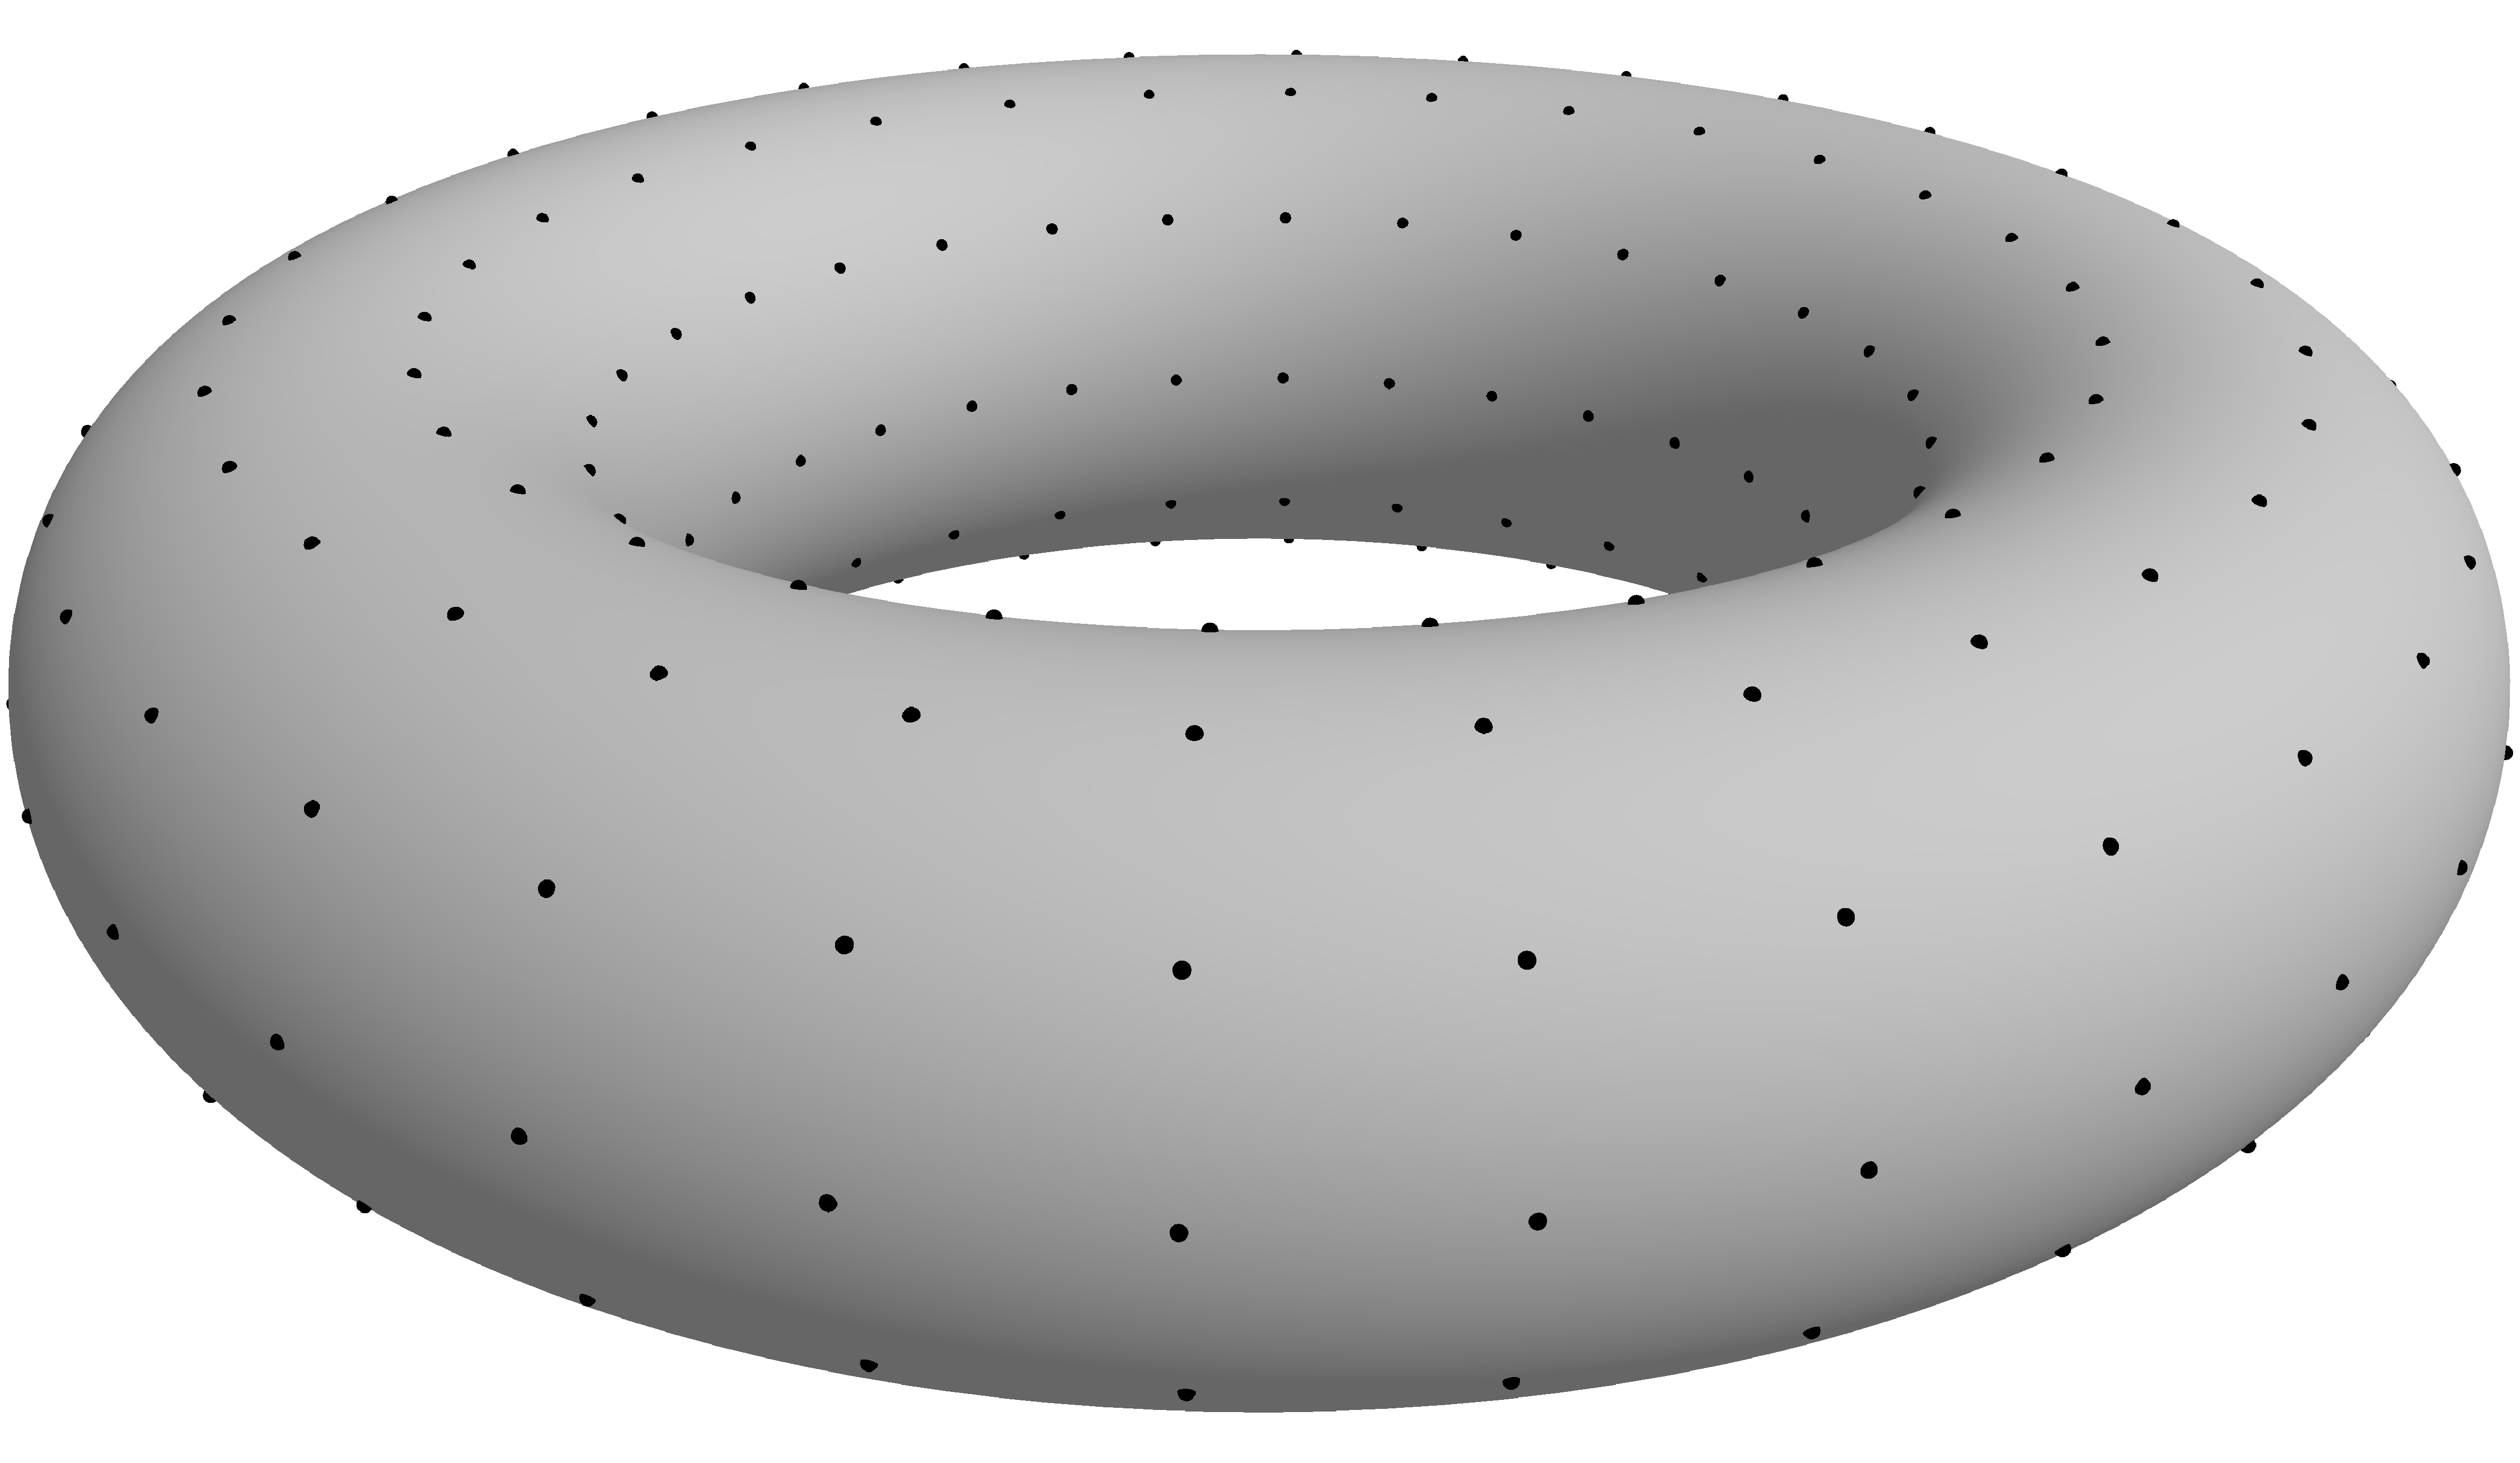
\includegraphics[width=3cm]{torus-with-net}
\end{center}
\par\noindent{}A metric space is \emph{totally bounded} if, for any \(\varepsilon > 0\), the metric space admits a finite open cover by balls of radius \(\varepsilon\); in other words, there is a finite \(\varepsilon\)-net for every \(\varepsilon>0\).
The proof of theorem~\vref{theorem:HB.naive} proves that compact metric spaces are totally bounded.
\begin{problem}{metric.spaces:tot.bdd.discrete}
Which discrete metric spaces are totally bounded?
\end{problem}
\begin{problem}{metric.spaces:tot.bdd.r}
In \(\R{n}\) with the standard discrete metric, are bounded sets totally bounded? the taxi-cab metric? the Euclidean metric? the sup norm metric?
\end{problem}
\begin{theorem}[Heine--Borel\define{Heine--Borel theorem}\define{theorem!Heine--Borel}]\label{theorem:h.b}
In a metric space, a set is compact just when it is complete and totally bounded.
\end{theorem}
\begin{proof}
Compact sets are complete and totally bounded.
Take a complete and totally bounded set.
Take any open cover of the set.
Pick a number \(\varepsilon_1 > 0\).
By total boundedness, we can cover our set in finitely many balls of radius \(\varepsilon\).
Suppose that each of these balls admits a finite cover by our open sets.
Then throw those finitely many covers together to cover the whole set, a finite subcover.
So we can suppose that there is one of these balls, say \(\ball{\varepsilon_1}{x_1}\), which is not covered by any finite number of our open sets.
Cover that ball by finitely many balls of a much smaller radius \(\varepsilon_2\), and conclude by the same reasoning that there is a ball, say \(\ball{\varepsilon_2}{x_2}\), which is not covered by any finite number of our open sets, with \(d\of{x_1,x_2}<\varepsilon_1\).
Inductively, generate a Cauchy sequence \(x_1, x_2, \dots\).
Replace with a subsequence to ensure convergence, say to some point \(x\).
But \(x\) is covered by one of our open sets, so therefore all points close enough to \(x\) are as well.
So one of the balls \(\ball{\varepsilon_j}{x_j}\) lies in that open set, a contradiction.
\end{proof}
A metric space is \emph{locally compact}\define{locally compact!metric space}\define{metric!space!locally compact} if every point lies in the interior of a compact set, and \emph{proper}\define{proper!metric space}\define{metric!space!proper} if every closed ball is compact.
Proper spaces are locally compact.
\begin{problem}{metric.spaces:proper}
Give an example of an improper locally compact metric space.
\end{problem}
\begin{answer}{metric.spaces:proper}
Any infinite set with standard discrete metric: balls of radius 2 are not compact, because the open cover by balls of radius \(1/2\) has no finite subcover, so not all balls are compact.
But the closed balls of radius \(1/2\) are compact, each being just a single point.
\end{answer}
\section{Compactness radius}
The \emph{compactness radius}\define{compactness radius}\define{radius!compactness} of a point \(x \in X\) in a metric space \(X\) is the supremum radius of a compact closed ball around \(x\), zero if there no such ball, infinite if balls of all radii about \(x\) are compact.
\begin{problem}{metric.spaces:radius.cpt.plane}
Find the compactness radius of a point \((x,y) \in X=\R{2}-\left\{(0,0)\right\}\) with metric induced from the Euclidean metric.
\end{problem}
\begin{problem}{metric.spaces:radius.cpt.1}
Prove that if a closed ball lies in a compact closed ball, then it is compact.
\end{problem}
\begin{problem}{metric.spaces:radius.cpt}
Prove that the compactness radius satisfies \(r(y) + d(x,y) \ge r(x)\) for any two points \(x\) and \(y\).
\end{problem}
\begin{answer}{metric.spaces:radius.cpt}
%\begin{center}
\begin{tikzpicture}[scale=.4]
\fill[gray!15] (0,0) circle (1cm);
\fill[gray!25] ({.75*cos(30)},{.75*sin(30)}) circle (.25cm);
\end{tikzpicture}
%\end{center}
\end{answer}
\begin{problem}{metric.spaces:radius.cpt.3}
Prove that the compactness radius is finite at one point just when it is finite at all points.
Prove that the compactness radius is positive everywhere just when the metric is locally compact. Prove that the compactness radius is infinite somewhere, and therefore everywhere, just when the metric is proper.
\end{problem}
\begin{answer}{metric.spaces:radius.cpt.3}
Immediate from \(r(y) + d(x,y) \ge r(x)\): if \(r(x)\) is infinite then so is \(r(y)\).
\end{answer}
\begin{problem}{metric.spaces:radius.cpt.2}
Prove that the compactness radius is continuous if finite.
\end{problem}
\begin{answer}{metric.spaces:radius.cpt.2}
In problem~\vref{problem:metric.spaces:radius.cpt} we saw that \(r(y)+d(x,y) \ge r(x)\), and by symmetry \(r(x)+d(x,y) \ge r(y)\).
Therefore \(d(x,y) \ge |r(x)-r(y)|\), so that if we make \(y \to x\), we find \(r(y) \to r(x)\).
\end{answer}
\begin{problem*}{metric.spaces:radius.cpt.4}
Prove that every connected, locally compact metric space is a countable union of compact sets.
\end{problem*}
\begin{answer}{metric.spaces:radius.cpt.4}
If the compactness radius is somewhere infinite, the space is proper, so its balls of positive integer radius are compact, and it is the union of these.
So assume that the compactness radius is everywhere finite.
By local compactness, the compactness radius is everywhere positive and \(d(x,y)\ge|r(x)-r(y)|\), so the compactness radius is continuous.
Taking any compact set \(K \subset X\), let \(K'\) be the union of all closed balls of radius \(r(x)/2\) about points \(x \in K\).
Any infinite sequence \(x_1,x_2,\dots \in K'\) has each \(x_i\) at distance at most \(r(y_i)/2\) from some \(y_i \in K\).
Take a convergent subsequence of \(y_1,y_2,\dots\), and replace the original sequence with the subsequence, so \(y_1,y_2,\dots \to y\) say.
Then \(d(x_i,y_i)\le r(y_i)/2 \to r(y)/2\).
Far enough down the sequence \(x_1,x_2,\dots\), every \(x_i\) lies in the compact ball of radius \(3r(y)/2\) about \(y\).
Thus \(x_1,x_2,\dots\) has a convergent subsequence.
\end{answer}

\section{Density}
A subset \(A \subset X\) of a metric space is \emph{dense}\define{dense} in another subset \(B\) if the closure of \(A\) contains \(B\), and \emph{everywhere dense}\define{everywhere dense}\define{dense!everywhere} if \(A\) is dense in \(X\).
A metric space is \emph{separable} if it contains a dense sequence of points.
\begin{example}
The rational numbers are dense in the real numbers.
\end{example}
\begin{example}
For each rational number \(q \in \Q{}\), take the set \(U_q \defeq \set{x \in \R{}|x \ne q}\).
So the various \(U_q \subset \R{}\) are dense open sets.
Their intersection 
\[
\bigcap_{q \in \Q{}} U_q \subset \R{}
\]
is precisely the set of irrational numbers, not open, but still dense.
Roughly speaking, if we only pull out a single rational at each step, we still have a lot left over after an infinite sequence of steps.
\end{example}
A set \(A \subset X\) in a metric space is \emph{nowhere dense}\define{dense!nowhere}\define{nowhere dense} if, for any open set \(U \subset X\), \(A \cap U\) is not dense in \(U\).
\begin{example}
The integers are nowhere dense in the real numbers.
\end{example}

\section{The Baire category theorem}
A \emph{meager set} is a subset \(S \subset X\) of a metric space, 
which can somehow be written as
\[
S = C_1 \cup C_2 \cup \dots
\]
as the union of a sequence of nowhere dense closed sets.
\begin{example}
For each rational number \(q \in \Q{}\), take the set \(\set{q} \subset \R{}\).
The various \(\set{q} \subset \R{}\) are nowhere dense closed sets.
Their union, \(\Q{}\), is dense, and not closed, but is still not ``very large'': it has dense complement.
\end{example}
A \emph{comeager}\define{comeager} set is a subset \(A \subset X\) of a metric space, which can somehow be written as
\[
A = U_1 \cap U_2 \cap \dots
\]
as the intersection of a sequence of dense open sets.
\begin{problem}{metric.spaces:comeager}
Prove that a subset of a metric space is meager just when its complement is comeager.
\end{problem}
\begin{theorem}[Baire category theorem]\label{theorem:Baire.category}\define{Baire category theorem}\define{theorem!Baire category}
In any complete metric space, every meager set has dense complement.
In other words, in any complete metric space, every comeager set is dense.
\end{theorem}
\begin{proof}
Take a comeager set
\[
A = U_1 \cap U_2 \cap \dots
\]
Since \(U_1\) is open, it contains a ball.
Since \(U_2\) is open and dense, it contains a ball nested inside the previous ball, and so on.
The Cauchy sequence of centers of the balls \(x_1, x_2, \dots\) converges, say to \(x \in X\).
Since the balls are nested, the point \(x\) is inside all of them.
So the intersection is not empty.

Pick a point \(x \in X\).
Since \(U_1\) is open and dense, it contains balls of radii as small as we like and as close as we like to \(x\).
For any one of these balls, we start the process of the previous paragraph, generating a point of the intersection inside that ball.
Changing the choice of ball, we can make those points approach \(x\).
\end{proof}
\begin{example}
Any countable subset \(S \subset \R{}\) of real numbers has dense complement.
Proof: The complete metric space \(X=\R{}\) contains the nowhere dense closed sets \(\set{x}\) for each point \(x\) of \(X\). 
Apply the Baire category theorem to any sequence of these.
\end{example}
\begin{example}
Take a sequence of polynomial functions \(p_1(x,y), p_2(x,y), \dots\) in two variables \(x,y\), each function nonzero somewhere.
Associate to each polynomial \(p_j(x,y)\) its set of zeroes \(V_j\defeq\set{(x,y)|p_j(x,y)=0}\).
The complete metric space \(X=\R{2}\) contains the nowhere dense closed sets \(V_j\).
By the Baire category theorem, the union
\[
S \defeq V_1 \cup V_2 \cup \dots
\]
has dense complement: you can avoid satisfying \emph{all} of the polynomial equations \(p_j(x,y)=0\) by slight perturbation of any point \((x,y) \in \R{2}\).
\end{example}
\begin{problem}{metric.spaces:Q.metric}
Suppose that we pick a metric on the set \(X \subset \R{}\) of all rational numbers, perhaps not the usual metric.
Suppose that the open sets of this metric are the usual open sets, as from the usual metric.
Prove that \(X\) is not complete.
\end{problem}
\begin{problem}{metric.spaces:no.isolated}
Suppose that \(X\) is a metric space with no isolated points.
Prove that \(X\) is incomplete or uncountable.
\end{problem}

\chapter{Maps of Metric Spaces}\label{chapter:maps.of.metric.spaces}
\chapterSummary{We prove some big theorems about continuous maps between metric spaces.}
\section{Continuity}
A map \(f \colon X \to Y\) between metric spaces is \emph{continuous}\define{continuous} if the inverse image of any open set is an open set.
For clarity we often denote the metric of a metric space \(X\) as \(d_X\) rather than \(d\).
\begin{problem}{metric.spaces:continuity}
Prove that a map \(f \colon X \to Y\) is continuous just when, for every point \(x_0 \in X\), and for every number \(\varepsilon > 0\), there is a number \(\delta > 0\) so that, for any point \(x_1 \in X\), if \(d_X\of{x_0,x_1}<\delta\) then \(d_Y\of{f\of{x_0},f\of{x_1}}<\varepsilon\).
\end{problem}
\begin{problem}{metric.spaces:continuity.discrete}
Suppose that \(X\) is a discrete metric space.
What are all continuous maps \(X \to \R{}\)?
What are all continuous maps \(\R{} \to X\)?
\end{problem}
\begin{problem}{metric.spaces:continuity.taxi}
Let \(X=\R{n}\) with the taxi-cab\SubIndex{taxi-cab metric}\SubIndex{metric!taxi-cab} metric and \(Y=\R{n}\) with the sup norm metric and let \(f \colon X \to Y\) be the map \(f(x)=x\).
Is \(f\) continuous?
Is \(f^{-1}\) continuous?
\end{problem}
\begin{problem}{metric.spaces:cont.distance}
Suppose that \(X\) is a metric space.
Equip \(X \times X\) with any one of the metrics described on page~\pageref{item:product.metrics} for products of metric spaces.
Prove that the metric itself \(d_X \colon X \times X \to \R{}\) is a continuous map.
\end{problem}
\begin{problem}{metric.spaces:cpt.image}
For any continuous map \(f \colon X \to Y\) of metric spaces, prove that the image \(f(S)\) of any compact set \(S \subset X\) is compact.
\end{problem}
\begin{problem}{metric.spaces:max.min}
Prove that every continuous function on any compact metric space achieves a maximum value and a minimum value.
\end{problem}
\begin{problem}{metric.spaces:cpt.img}
Prove that every continuous map from a compact metric space to a metric space has compact image.
\end{problem}

\section{Uniform continuity}
Let \(X\) and \(Y\) be metric spaces.
A sequence of maps \(f_1, f_2, \dots \colon X \to Y\) \emph{converges pointwise}\define{convergence!pointwise}\define{pointwise!convergence} to a map \(f \colon X \to Y\) if, for any point \(x\), \(f_i(x) \to f(x)\).
\begin{exampleAndImage}{1.412cm}
On \([0,1]\), the functions \(f_j(x)=x^j\) converge pointwise to
\[
f(x)=
\begin{cases}
1, & \text{ if \(x=1\)}, \\
0, & \text{ otherwise}.
\end{cases}
\]
So a sequence of continuous functions can converge pointwise to a discontinuous function.
Picture how it happens: if we sit at any one point \(x < 1\), we watch while the functions \(x, x^2, \dots\) get smaller and smaller, going to zero.
But for larger \(x\) values, it takes  much longer for this too happen; we have to get further down to sequence keep all of the numbers \(x, x^2, \dots\) smaller than \(\varepsilon\).
\tcblower
\documentclass{standalone}
\usepackage{pgfplots}
\begin{document}
\begin{tikzpicture}
\pgfplotsset{width=3cm}
\begin{axis}[axis lines=none,scaled ticks=false,mark=none]
\addplot[gray!100!white,domain=0:1,samples=201]{x^2};
\addplot[gray!80!white,domain=0:1,samples=201]{x^4};
\addplot[gray!60!white,domain=0:1,samples=201]{x^8};
\addplot[gray!40!white,domain=0:1,samples=201]{x^(16)};
\addplot[gray!20!white,domain=0:1,samples=201]{x^(32)};
\end{axis}
\end{tikzpicture}
\end{document}

\end{exampleAndImage}
The \emph{uniform distance}\define{uniform!distance} between two maps \(f,g \colon X \to Y\) is
\[
d(f,g)=\sup_{x \in X}d_Y\of{f(x),g(x)}.
\]
Warning: if \(X\) is not compact, and \(Y\) is not bounded, there might be infinite uniform distance between two maps.
\begin{exampleAndImage}{2.415cm}
The uniform distance between \(y=x\) and \(y=\sin x\) (where \(X=Y=\R{}\)) is infinite because the linear function grows arbitrarily large, while the sine function stays bounded.
\tcblower
\documentclass{standalone}
\usepackage{pgfplots}
\begin{document}
\begin{tikzpicture}
\pgfplotsset{width=4cm}
\begin{axis}[axis lines=none,scaled ticks=false]
\addplot[gray,domain=0:10,samples=201]
{sin(deg(x))};
\addplot[gray!50!white,domain=0:10,samples=201]
{x};
\end{axis}
\end{tikzpicture}
\end{document}

\end{exampleAndImage}
\begin{exampleAndImage}{1.42cm}
The sequence \(x, x^2, x^3, \dots\) on \(X=[0,1]\) converges  pointwise  to
\[
f(x)=
\begin{cases}
1, & \text{ if \(x=1\)}, \\
0, & \text{ otherwise},
\end{cases}
\]
but not uniformly.
Any particular function \(x^k\) will be almost one unit away from zero for \(x\) close enough to \(1\), so the uniform distance is \(d\of{x^k,f}=1\) for all \(k=1,2,\dots\).
\tcblower
\documentclass{standalone}
\usepackage{pgfplots}
\begin{document}
\begin{tikzpicture}
\pgfplotsset{width=3cm}
\begin{axis}[axis lines=none,scaled ticks=false,mark=none]
%\addplot[gray!100!white,domain=0:1,samples=201]{x^2};
%\addplot[gray!80!white,domain=0:1,samples=201]{x^4};
%\addplot[gray!60!white,domain=0:1,samples=201]{x^8};
\draw[brown!50!white, thick] (axis cs: {.93},0) -- (axis cs: {.93},{(.93)^8});
\addplot[gray!60!white,thick,domain=0:1,samples=201]{x^8};
%\addplot[gray!20!white,domain=0:1,samples=201]{x^(32)};
\draw[blue!40!gray,thick] (axis cs: 0,0) -- (axis cs: 1,0) -- (axis cs: 1,1);
\end{axis}
\end{tikzpicture}
\end{document}

\end{exampleAndImage}
\begin{center}
\documentclass{standalone}
\usepackage{pgfplots}
\begin{document}
\begin{tikzpicture}
\pgfplotsset{width=4cm}
\begin{axis}[axis lines=none,scaled ticks=false]
\addplot[gray,domain=0:3.14159,samples=201]
{sin(deg(x))^2};
\addplot[gray!90!white,domain=0:3.14159,samples=201]
{sin(deg(x))^2+0.06*sin(20*deg(x))+0.04*cos(35*deg(x))};
\addplot[blue!50!white,domain=0:3.14159,samples=201]
{sin(deg(x))^2+0.1};
\addplot[blue!50!white,domain=0:3.14159,samples=201]
{sin(deg(x))^2-0.1};
\end{axis}
\end{tikzpicture}
\end{document}

\end{center}
A sequence of maps \(f_1, f_2, \dots \colon X \to Y\) \emph{converges uniformly}\define{convergence!uniform}\define{uniform!convergence} to a map \(f \colon X \to Y\) if the uniform distance from \(f_i\) to \(f\) converges to zero.
A sequence of maps \(f_1, f_2, \dots \colon X \to Y\) is \emph{uniformly Cauchy}\define{uniformly!Cauchy}\define{Cauchy!uniformly} if the uniform distances between \(f_i\) and \(f_j\) converge to zero as \(i, j \to \infty\).
\begin{example}
Take a little bump
\inputinexample{uniform-convergence-on-compact-sets-start}
and slide it along
\inputinexample{uniform-convergence-on-compact-sets}
as a sequence of functions \(f_1, f_2, \dots\), so that the bump flies off to infinity.
If you sit at any one point long enough, you watch the bump fly past, and then the functions settle down toward zero.
Every function in this sequence has the same height, and so the distance to the zero function always stays the same.
So the uniform distance from the zero function is always the same positive number: \(f_1, f_2, \dots\) does not converge uniformly.
If you fix any finite interval and watch the functions \(f_1, f_2, \dots\) along that interval, they converge rapidly to \(0\) uniformly along that interval: uniform convergence on compact sets.
\end{example}
A sequence of maps \(f_1, f_2, \dots \colon X \to Y\) is \emph{locally uniformly Cauchy}\define{locally uniformly!Cauchy}\define{Cauchy!locally uniformly} if every point of \(X\) lies in an open set in which the uniform distances between \(f_i\) and \(f_j\) converge to zero as \(i, j \to \infty\).
\begin{example}
The functions \(f_j \colon \R{} \to \R{}\), \(f_j(x)=x^j/j!\) are locally uniformly Cauchy, but not uniformly Cauchy.
\end{example}
\begin{problem}{metric.space.maps:arctan}
Draw pictures to explain why the functions \(f_j \colon \R{} \to \R{}\), \(f_j(x)=2\arctan(jx)/\pi\) are pointwise Cauchy, but are not locally uniformly Cauchy in any open set containing the origin.
\end{problem}
\begin{answer}{metric.space.maps:arctan}
\begin{center}
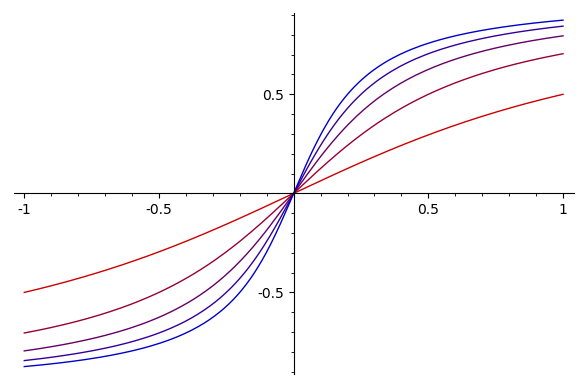
\includegraphics[width=5cm]{arctan-plots}
\end{center}
\end{answer}
\begin{lemma}\label{lemma:complete.converg}
Any locally uniformly Cauchy sequence of maps \(f_1, f_2, \dots \colon X \to Y\) between metric spaces which converges pointwise converges to a continuous map.
In particular, if \(Y\) is a complete metric space, then any locally uniformly Cauchy sequence of maps \(f_1, f_2, \dots \colon X \to Y\) converges to a continuous map.
\end{lemma}
\begin{proof}
Take a locally uniformly Cauchy sequence of maps \(f_1, f_2, \dots \colon X \to Y\).
Cover \(X\) by open sets in which the convergence is uniformly Cauchy.
It suffices to show that the restrictions of these maps to those open sets converge to a continuous map.
So we can assume that the convergence is uniformly Cauchy.

If \(Y\) is complete, then for each point \(x \in X\), the values \(f_1(x), f_2(x), \dots \in Y\) form a Cauchy sequence, so converge, say to some point \(f(x) \in Y\).
So we can assume pointwise convergence.

Pick some point \(x_0 \in X\) and some \(\varepsilon > 0\).
Let \(y_0=f\of{x_0}\) and let \(y_i=f_i\of{x_0}\).
If we take \(i\) large enough we can get \(d\of{f_i,f}\) as small as we like, i.e. \(d\of{f_i(x),f(x)}\) is small for all \(x\).
Once we fix that value of \(i\), for every \(x\) close enough to \(x_0\), \(d\of{f_i(x),y}\) is as small as we like.
So 
\[
d\of{y_0,f\of{x}} 
\le 
d\of{y_0,y_i} 
+
d\of{y_i,f_i\of{x}} 
+
d\of{f_i\of{x},f\of{x}} 
\]
is as small as we like, so \(f\) is continuous.
\end{proof}
Let \(F\) be the set of continuous maps \(f \colon X \to Y\) between two metric spaces \(X\) and \(Y\).
We try to turn \(F\) into a metric space by taking the \emph{uniform metric}\define{uniform!metric}\define{metric!uniform} to be given by the uniform distance.
If \(F\) is compact, or \(F\) is bounded, then \(F\) is a metric space.
More generally, pick a particular continuous map \(f \colon X \to Y\) as ``origin''; the set \(F_f\) of continuous maps \(g\) of uniformly bounded distance from \(f\), i.e. with finite value for \(d(f,g)\), is a metric space.
\begin{example}
If \(f\) is bounded, then \(F_f\) is the set of all bounded continuous maps \(X \to Y\).
\end{example}
\begin{example}
If \(f(x)=e^x\) is the exponential function (and again \(X=Y=\R{}\)), then \(F_f\) is the set of functions \(e^x+b(x)\) where \(b(x)\) is any bounded continuous function.
\end{example}
\begin{corollary}\label{corollary:Zf}
Pick a continuous map \(f \colon X \to Y\) from a metric space \(X\) to a complete metric space \(Y\).
The set of all continuous maps of bounded uniform metric distance from \(f\) is a complete metric space in the uniform metric.
\end{corollary}

\section{Equicontinuity}
A set \(F\) of continuous maps \(X \to Y\) is \emph{equicontinuous}\define{equicontinuous} if for every \(x \in X\) and every \(\varepsilon > 0\), \(x\) lies in an open set \(U_x \subset X\) such that for any \(y \in U_x\) and \(f \in F\), \(d(f(x),f(y)) < \varepsilon\); in other words, if we move \(x\) only a little bit, to a nearby point \(y\), all of the functions in \(F\) change only a little.
\begin{problem}{metric.spaces:equi}
Is the sequence \(x,x^2,x^3,\dots\) equicontinuous on \([0,1]\)? On \((0,1)\)?
\end{problem}
\begin{problem}{metric.spaces:equi.disc}
If \(X\) and \(Y\) are metric spaces, and \(X\) is discrete, which sets \(F\) of maps \(X \to Y\) are equicontinuous?
\end{problem}
A set \(F\) of continuous maps is \emph{pointwise bounded}\define{pointwise!bounded}\define{bounded!pointwise} or \emph{pointwise totally bounded}\define{bounded!pointwise!totally}\define{pointwise!bounded!totally} or \emph{pointwise relatively compact}\define{pointwise!relatively compact}\define{relatively!compact!pointwise} if for every \(x \in X\), the set \(\Set{f(x)|f \in F} \subset Y\) is bounded or totally bounded or relatively compact.
\begin{theorem}[Arzel\'a--Ascoli I]\label{theorem:Arzela.Ascoli.I}\define{theorem!Arzela--Ascoli@Arzel\'a--Ascoli}
Let \(X\) be a compact metric space and \(Y\) a metric space. 
Take a set \(F\) of continuous maps \(X \to Y\).
Then the following properties of \(F\) are equivalent:
\begin{enumerate}
\item 
The set \(F\) is equicontinuous and pointwise relatively compact,
\item
Every infinite sequence of maps \(f_1, f_2, \dots \in F\) has a convergent subsequence.
\end{enumerate}
\end{theorem}
\begin{proof}
Pick any \(\varepsilon > 0\). 
Since \(F\) is equicontinuous, every point \(x \in X\) lies in an open set \(U_x \subset X\) in which 
\[
d(f(s),f(t)) < \frac{\varepsilon}{4},
\]
for all \(s,t \in U_x\) and \(f \in F\).
Since \(X\) is compact, we can choose a finite subcover \(U_{x_1}, U_{x_2}, \dots, U_{x_n}\).
Because \(F\) is pointwise relatively compact, the set of points \(f\of{x_1}, f\of{x_2}, \dots, f\of{x_n}\) is a relatively compact subset of \(Y\).
So we can pick some points \(y_1, y_2, \dots, y_m \in Y\) so that every point \(f\of{x_i}\) lies within distance \(\frac{1}{4}\varepsilon\) from one of these \(y_j\).
Let \(F'\) be the set of all maps
\[
\phi \colon \Set{x_1, x_2, \dots, x_n} \to \Set{y_1, y_2, \dots, y_m},
\]
a ``discrete  approximation'' of \(F\).
For each \(\phi \in F'\), let  
\[
F_{\phi} = \Set{f \in F| d\of{f\of{x_i},\phi\of{x_i}} < \frac{\varepsilon}{4}, i=1,2,\dots,n}.
\]
Then \(F\) is the union of all sets \(F_{\phi}\), for all maps \(\phi \in F'\).

First we want to prove that each \(F_{\phi}\) has diameter at most \(\varepsilon\) in the uniform metric, so it essentially like a small ball around the point \(\phi\) in our discrete approximation.
If \(f, g \in F_{\phi}\), then \(d(f,\phi)<\frac{\varepsilon}{4}\) and \(d(g,\phi)<\frac{\varepsilon}{4}\) on \(x_1, x_2, \dots, x_n\).
So then \(d(f,g) < \frac{\varepsilon}{2}\) on \(x_1, x_2, \dots, x_n\).
But then for any \(x \in X\), \(x \in U_{x_i}\) for some \(i\) so
\begin{align*}
d(f(x),g(x)) 
&\le
d\of{f(x),f\of{x_i}} 
+
d\of{f\of{x_i},g\of{x_i}} 
+
d\of{g\of{x_i},g(x)},
\\
&\le 
\varepsilon.
\end{align*}
So effectively we have found a ``discrete approximation'' \(F'\) to  \(F\), and \(F\) looks like a collection of small balls around those discrete points.

Picking one map \(f\) from every nonempty \(F_{\phi}\), for every \(\phi \in F'\), we obtain a finite set of maps \(F_{\varepsilon}\) so that every map in \(F\) lies within distance \(\varepsilon\) of one of them, an \(\varepsilon\)-net\SubIndex{net} inside \(F\).
In particular, \(F\) is totally bounded, so lies inside some space \(F_f\) of maps of uniformly bounded distance from a single map \(f\).
If we replace \(F\) by its closure in \(F_f\), we still have equicontinuity and pointwise relative compactness, so we can assume that \(F\) is closed and totally bounded.

Take a sequence \(\varepsilon_1, \varepsilon_2, \dots \to 0\) and for each \(\varepsilon_i\) cover \(X\) by all open balls of radius \(\varepsilon_i\), and then take a finite subcover.
The center points of the balls in those finite subcovers, all put together, form a dense countable subset of \(X\), say \(x_1, x_2, \dots\).
For any sequence \(f_1, f_2, \dots \in F\), take a subsequence whose values converge at \(x_1\), and out of that a further subsequence whose values converge at \(x_2\), and so on.
Take the first entry from the \(n\)-th subsequence whose value at \(x_1, x_2, \dots, x_n\) is within \(\varepsilon_n\) of the limit value.
So we have a subsequence converging on a dense subset.
By equicontinuity, the same subsequence converges near each point of the dense subset, i.e. everywhere.
\end{proof}
\begin{theorem}[Arzel\'a--Ascoli II]\label{theorem:Arzela.Ascoli.II}\define{theorem!Arzela--Ascoli@Arzel\'a--Ascoli}
Suppose that \(X\) and \(Y\) are metric spaces and that \(X\) is proper.
Then every equicontinuous and pointwise relatively compact sequence of maps \(f_1, f_2, \dots \colon X \to Y\) has a subsequence converging uniformly on compact sets of \(X\) to a continuous map \(f \colon X \to Y\).
\end{theorem}
\begin{proof}
Let \(\bar{B}_k\) be the ball in \(X\) of radius \(k\) about some point \(x_0 \in X\).
By properness, these balls are compact.
Pick some sequence of positive numbers \(\varepsilon_1, \varepsilon_2 \to 0\).
By theorem~\vref{theorem:Arzela.Ascoli.I}, on \(\bar{B}_1\) some subsequence of these \(f_n\) converge to some map \(f\).
Pick one element of that subsequence which lies within distance \(\varepsilon_1\) of the limit, uniformly on \(\bar{B}_1\), and call it \(g_1\).
By theorem~\vref{theorem:Arzela.Ascoli.I}, on \(\bar{B}_1\) some subsequence of that subsequence converges to some map, necessarily agreeing on \(\bar{B}_1\) with the map \(f\) we already defined.
Pick one element of that subsubsequence which lies within distance \(\varepsilon_2\) of the limit, uniformly on \(\bar{B}_2\),and call it \(g_2\).
Repeat inductively.
\end{proof}

\section{Dilation}
A map \(f \colon X \to Y\) between metric spaces is \emph{distance preserving}%
\define{distance!preserving map}%
\define{map!distance preserving} 
if \(d_Y\of{y_0,y_1}=d_X\of{x_0,x_1}\) whenever \(y_0=f\of{x_0}\) and \(y_1=f\of{x_1}\), for any points \(x_0, x_1 \in X\).
An \emph{isometry}\define{isometry} is a distance preserving bijection; its inverse is then also an isometry.
A subset \(S \subset X\) of a metric space is \emph{dense}\define{dense} if the closure of \(S\) is \(X\).
\begin{problem}{metric.spaces:dense.Q}
Prove that the rational numbers are dense in the real numbers with Euclidean metric.
\end{problem}
\begin{problem}{metric.spaces:dense}
Suppose that \(S \subset X\) and \(T \subset Y\) are subsets of complete metric spaces and that \(S \subset X\) is dense.
Prove that every distance preserving map \(S \to T\) of the induced metrics extends uniquely to a distance preserving map \(X \to Y\).
\end{problem}
\begin{problem}{metric.spaces:balls.iso}
Suppose that \(X\) and \(Y\) are metric spaces, \(x_0\) a point of \(X\) and \(y_0\) a point of \(Y\), and that, for every real number \(r\), \(\ball[X]{r}{x_0}\) is isometric to \(\ball[Y]{r}{y_0}\).
Is \(X\) isometric to \(Y\)?
\end{problem}
The \emph{dilation}\define{dilation} of a map \(f \colon X \to Y\) between metric spaces is 
\[
\sup_{x_0 \ne x_1}
\frac{d_Y\of{f\of{x_0},f\of{x_1}}}{d_X\of{x_0,x_1}}
\]
(which can be \(\infty\)).
A \emph{Lipschitz}\define{Lipschitz} map is a map of finite dilation.
\begin{problem}{metric.space.maps:Lipschitz}
Which are Lipschitz: \(|x|, |x|^{1/2}, x^{1+\varepsilon} \sin(1/x)\)?
\end{problem}
\begin{problem}{metric.space.maps:Lipschitz.distance}
Fix a point \(x_0 \in X\) in a metric space and let \(r(x)=d\of{x_0,x}\).
Prove that \(r\) has unit dilation.
\end{problem}
\begin{problem*}{metric.spaces:wedding.blanket}
Prove the wedding blanket theorem:\define{wedding blanket theorem}\define{theorem!wedding blanket} any map \(f \colon X \to X\) on a compact metric space so that \(d(f(x),f(y))\ge d(x,y)\) is an isometry.
\end{problem*}
\begin{problem}{metric.space.maps:Lipschitz.continuous}
A map has \emph{locally bounded dilation}\define{locally!bounded!dilation}\define{dilation!locally bounded} (also called a \emph{locally Lipschitz map})\define{Lipschitz!locally}\define{locally!Lipschitz} if its restriction to any bounded set has finite dilation.
Prove that maps of locally bounded dilation are continuous.
\end{problem}
\begin{proposition}\label{proposition:locally.bounded.dilation}
A map \(S \to Y\) of locally bounded dilation from a dense subset \(S \subset X\) of a metric space to a complete metric space \(Y\) extends uniquely to a map \(X \to Y\) of locally bounded dilation, with the same local dilation bound.
\end{proposition}
\begin{proof}
It is enough to prove the result locally.
If \(x \in X\) is the limit of a sequence \(s_1, s_2, \dots \in S\), then \(f\of{s_i}\) is a Cauchy sequence, since \(f\) stretches distances by a bounded factor at most.
Let \(f(x)=\lim f\of{s_j}\).
If we have another sequence \(t_1, t_2, \dots \in S\) with limit \(x\), then \(s_i\) and \(t_j\) get and stay both close to \(x\), for large enough \(i\) and \(j\), so \(f\of{s_i}\) is close to \(f\of{t_j}\), since again \(f\) stretches distances by at most a bounded factor.
Therefore \(f(x)\) is well defined.
Again, since \(f\) stretches distances by at most a bounded factor on \(S\), taking limits gives the same factor, the same dilation.
\end{proof}
\begin{problem}{metric.spaces:smooth.dilation}
Suppose that \(X \subset \R{p}\) and \(Y \subset \R{q}\) are open subsets and that \(f \colon X \to Y\) is a continuously differentiable map.
Prove that the dilation of \(f\) is the supremum of \(\norm{f'(x)}\) for \(x \in X\).
\end{problem}

\section{Completion}
\begin{theorem}
Every metric space \(X\) is a dense subset of a complete metric space \(\bar{X}\).
The metric space \(\bar{X}\) is uniquely determined up to isometry.
\end{theorem}
\begin{proof}
Uniqueness: By density, if \(X \subset Y\) and \(X \subset Z\) is dense in two metric spaces, the idenity map \(X \to X\) uniquely extends to a continuous map \(Y \to Z\) of dilation at most 1 and in the same way to a continuous map \(Z \to Y\) of dilation at most 1, by proposition~\vref{proposition:locally.bounded.dilation}, hence both are isometries.

Existence: Intuitively, we picture that there are some ``missing'' points to \(X\), which we should fill in to get Cauchy sequences to converge.
\begin{example} If \(X\) is a disk punctured at a point:
\begin{center}
\documentclass[tikz]{standalone}
\begin{document}
\begin{tikzpicture}
\fill[gray!50] (0,0) circle (1cm);
\fill[white,draw=gray] (0,0) circle (1.4pt);
\end{tikzpicture}
\end{document}

\end{center}
we want \(\bar{X}\) to include that point.
We can ``feel'' that the point is ``missing'' from \(X\), because there are Cauchy sequences heading inward, with no limit in \(X\):
\begin{center}
\documentclass[tikz]{standalone}
\begin{document}
\begin{tikzpicture}
\newcount\myangle
\newcount\myradiusinverse
\fill[gray!50] (0,0) circle (1cm);
\foreach \i in {1,...,50}{
	\myangle=\i
	\multiply\myangle by 10
	\myradiusinverse=\i
	\fill[black] ({(.2*ln(\myradiusinverse)*cos(\myangle)},{.2*ln(\myradiusinverse)*sin(\myangle)}) circle (1pt);
}
\fill[white,draw=gray] (0,0) circle (1.4pt);
\end{tikzpicture}
\end{document}

\end{center}
\end{example}
Declare two Cauchy sequences \(x_1,x_2,\dots\) and \(y_1,y_2,\dots\) of points \(x_i, y_j \in X\) to be equivalent if the distances \(d\of{x_i,y_j} \to 0\) as \(i,j \to \infty\).
Let \(\bar{X}\) be the set of equivalence classes.
The ``distance'' between two Cauchy sequences \(x=(x_1,x_2,\dots)\) and \(y=(y_1,y_2,\dots)\) of points of \(X\) is
\[
\bar{d}\of{x,y}=\lim_{m,n \to \infty} \sup_{i>m,j>n} d\of{x_i,y_j}.
\]
This is \emph{not} a metric.
Clearly our ``distance'' between Cauchy sequences depends only on their equivalence class, so \(\bar{d}\) is defined on pairs of points of \(\bar{X}\).
If \(\bar{d}\of{x,y}=0\) then clearly the equivalence classes can only be represented by equivalent Cauchy sequences, so are equal.
Similarly, the triangle inequality just pulls out of the limit and supremum to give a triangle inequality on \(\bar{X}\).
Map \(X \to \bar{X}\) by taking each point \(x\) of \(X\) to the equivalence class of the constant sequence \(x,x,x,\dots\) in \(\bar{X}\).

We need to prove that \(\bar{X}\) is complete.
We take a Cauchy sequence \(x_1, x_2, \dots\) in \(\bar{X}\).
Each \(x_i\) is the equivalence class of a Cauchy sequence \(x_{i1}, x_{i2}, \dots\) in \(X\).
As we make \(i,j \to \infty\), \(\bar{d}\of{x_i,x_j} \to 0\).
This means that \(d\of{x_{ik},x_{jl}} \to 0\) as we make \(i,j,k,l \to \infty\).
In particular, if we let \(y_i\defeq x_{ii}\), then \(x_1, x_2, \dots\) converges to \(y\) in \(\bar{X}\).
\end{proof}

\section{Contraction maps}
A \emph{contraction}\define{contraction} is a map \(f \colon X \to X\) of dilation less than \(1\).
Given a map \(f \colon X \to X\) on a metric space, let \(f^{\circ 0} \colon X \to X\) be the identity map, and inductively let \(f^{\circ (n+1)}=f \circ f^{\circ n}\).
The map is a \emph{pinch}\define{pinch} if the sum \(\lambda_1+\lambda_2+\dots\) of the dilations \(\lambda_n\) of the  compositions \(f^{\circ n}\) is finite.
\begin{example}
Every map with dilation \(\lambda\) has \(\lambda_n \le \lambda^n\), so contractions pinch.
\end{example}
\begin{theorem}[Contraction mapping theorem\define{theorem!contraction mapping}\define{contraction!mapping theorem}]
Every pinch of a complete metric space has a unique fixed point.
If \(x_0\) is any point, and \(f\) a pinch, with dilation sum at most \(c\), let \(D\defeq d(x_0,f(x_0))\).
Then the fixed point is at most \(D(1+\lambda_1+\lambda_2+\dots)\) away from \(x_0\).
\end{theorem}
\begin{proof}
Let
\begin{align*}
x_1 &= f\pr{x_0}, \\
x_2 &= f\pr{x_1}, \\
&\vdots
\end{align*}
We want to prove that this sequence has a fixed point as limit. 
Imagine for the moment that we know the sequence is Cauchy. 
It converges, say to some point \(x\), so 
\[
x=\lim_{i \to \infty} f\pr{x_i}.
\]
The function \(f\) is continuous, so
\[
f\pr{\lim_{j \to \infty} x_j}
=
\lim_{j \to \infty} f\pr{x_j}.
\]
Therefore
\(
f(x)=x,
\)
a fixed point.

So we only need to prove that \(x_0,x_1, x_2, \dots\) is a Cauchy sequence. 
Let \(D\) be the distance  from \(x_0\) to \(x_1\). 
How fast do the distances shrink?
The sum of positive terms \(\lambda_1+\lambda_2+\dots\) is finite, so \(\lambda_i \to 0\) as \(i\to\infty\).
If \(m\) is the smaller of \(k,\ell\), and \(n=|k-\ell|\),
\begin{align*}
d(x_k,x_{\ell})
&\le
\lambda_m d(x_0,x_n),
\\
&\le
\lambda_m (d(x_0,x_1)+d(x_1,x_2)+\dots+d(x_{n-1},x_n)),
\\
&
\le
\lambda_m(1+\lambda_1+\lambda_2+\dots+\lambda_{n-1})D.
\end{align*}
As \(m\to \infty\), this vanishes, as \(\lambda_m\to 0\).
So this sequence is Cauchy.
The distance from \(x_0\) to the fixed point is bounded, by taking the limit.
\end{proof}
\begin{problem}{metric.space.maps:circle.maps}
Take the set \(X\) of all continuous maps \(f \colon S^1 \to S^1\) with the uniform metric.
It is clear by looking at the trigonometric functions and their inverse functions that \(f\) has a \emph{lift} (also called its \emph{angle function}),  a continuous function \(\hat{f} \colon \R{} \to \R{}\) so that \(f(e^{i\theta})=e^{i\hat{f}(\theta)}\).
The degree of \(f\) is 
\[
\frac{1}{2\pi}(\hat{f}(2\pi)-\hat{f}(0)).
\]
Approximate \(\hat{f}\) by a ``linear'' map as follows.
Take slope \(m\) equal to the degree of \(f\).
The intercept \(\beta_0\) is the average of \(\hat{f}(\theta)-m\theta\):
\[
\beta_0 = \frac{1}{2\pi} \int_0^{2\pi} \hat{f}(\theta) \, d\theta
-
\pi m.
\]
Associate to any continuous map \(f \colon S^1 \to S^1\) and number \(0 \le t \le 1\) the map \(F_t f\) whose lift is
\[
\theta \mapsto (1-t)\hat{f}(\theta)+t\pr{m\theta+\beta_0}.
\]
Prove that on continuous maps of the circle of a given degree, the map \(F_t\) is a contraction map if \(t>0\) and is continuous in \(t\).
\end{problem}
\begin{answer}{metric.space.maps:circle.maps}
Given two maps \(f, g \colon S^1 \to S^1\) of the circle, with equal degree, let \(f_t=F_t f\) and \(g_t=F_t g\). 
Then
\[
\hat{f}_t(\theta)-\hat{g}_t(\theta) = (1-t)\pr{\hat{f}(\theta)-\hat{g}(\theta)}
+\frac{t}{2\pi} \int_0^{2\pi} \hat{f}-\hat{g}.
\]
Therefore
\[
d\pr{f_t,g_t}
\le
(1-t)d\pr{f,g}.
\]
\end{answer}
\begin{center}
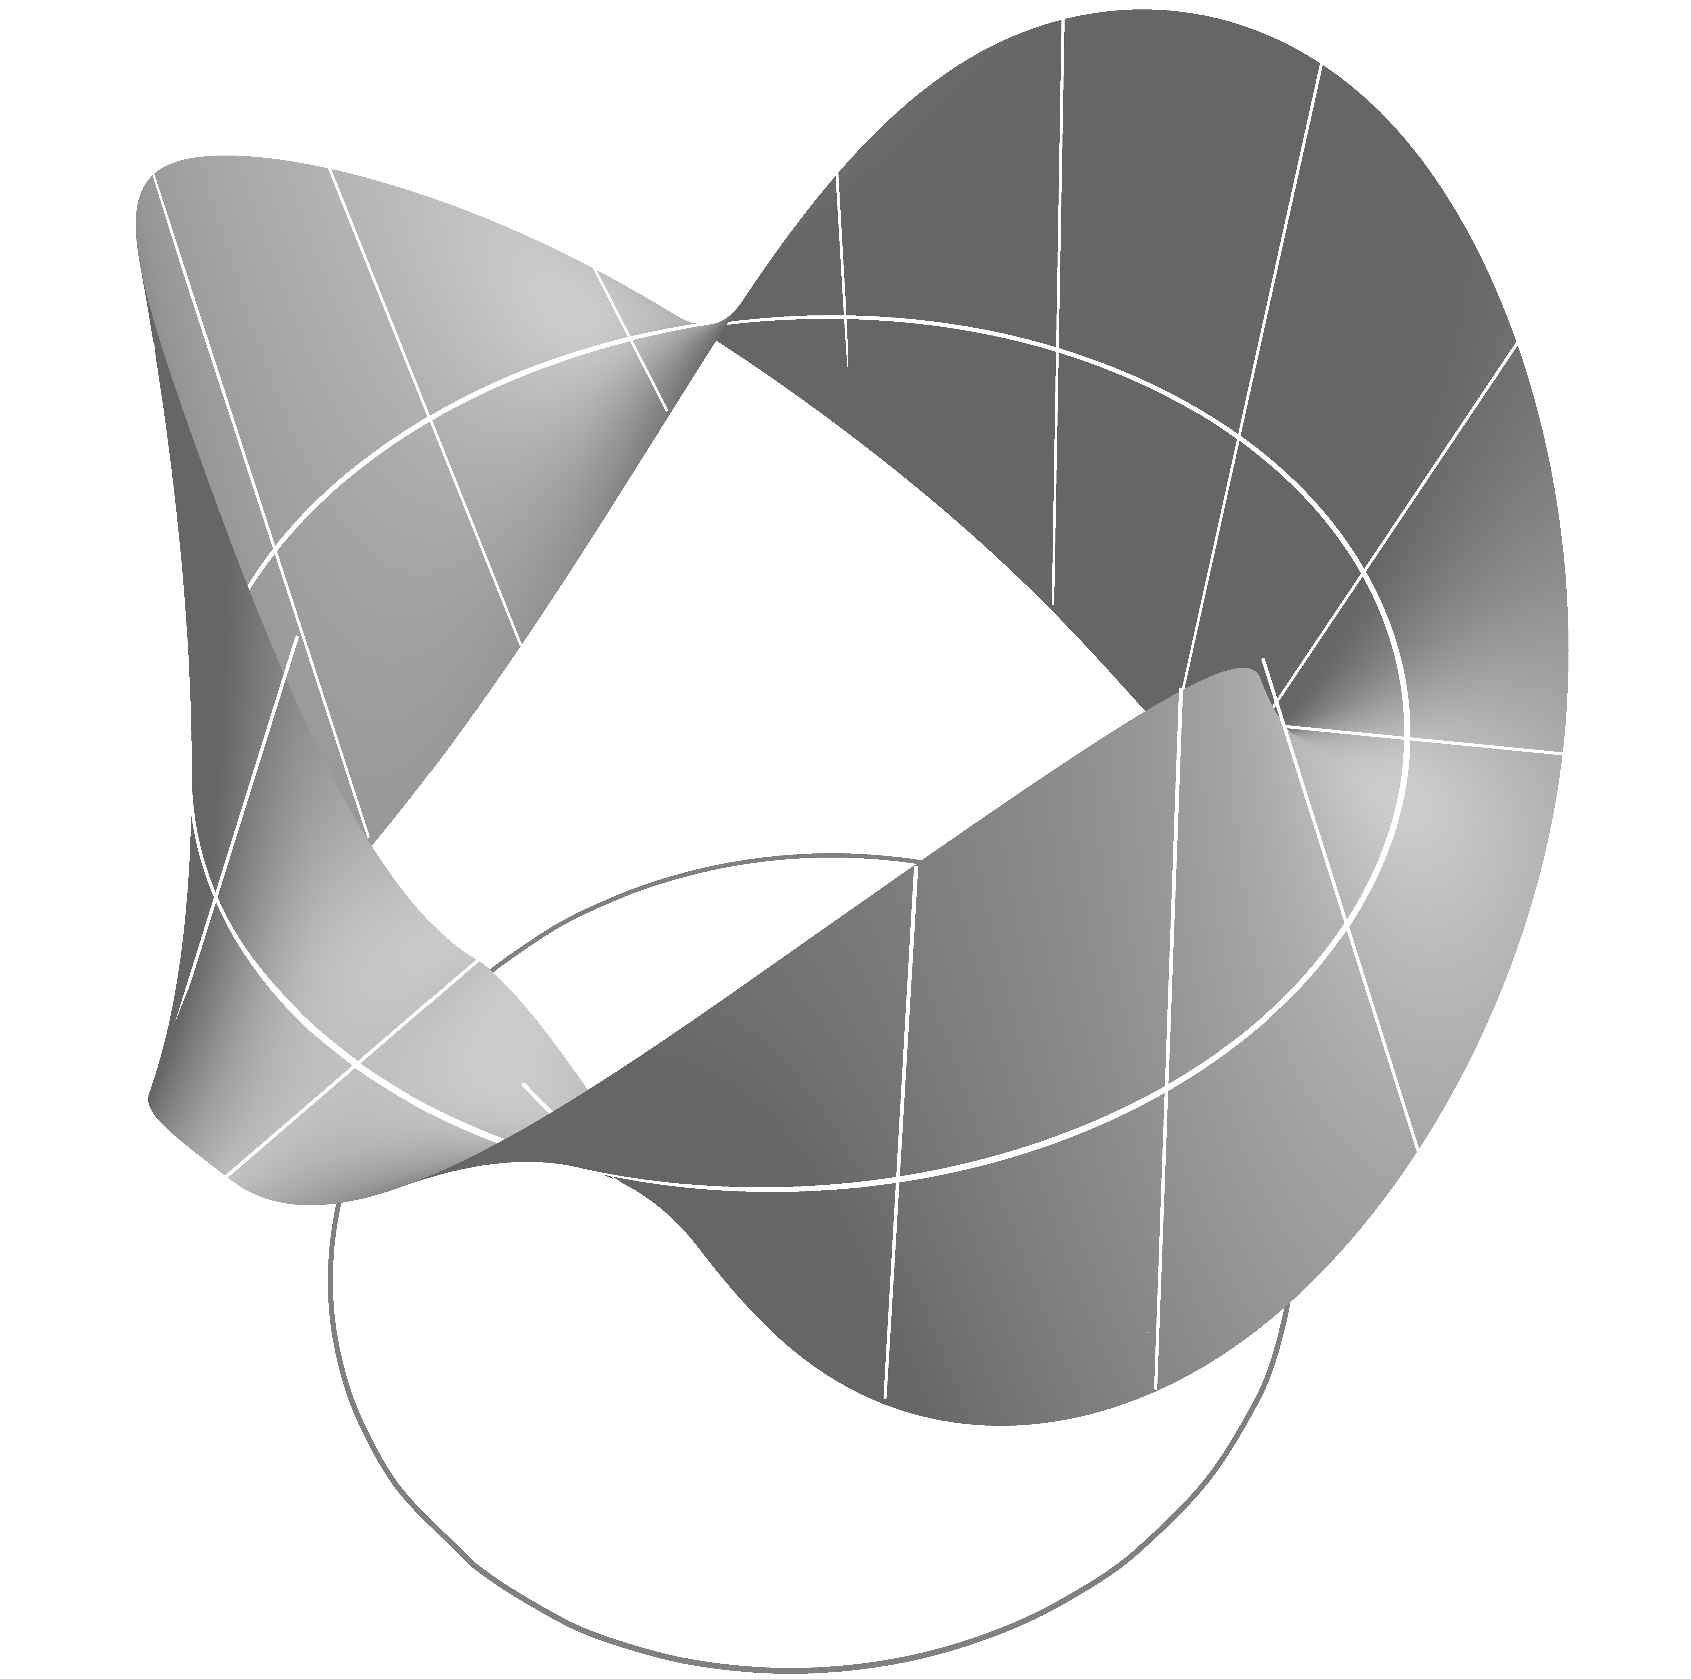
\includegraphics[width=5cm]{moebius-strip-as-bundle}
\end{center}
A \emph{family of metric spaces}\define{metric space!family}\define{family!metric spaces} is a surjective continuous map \(f \colon X \to Y\) of metric spaces.
The \emph{stalks}\define{stalk} of the map are the sets \(f^{-1}(y)\), which we denote as \(X_y\), for all \(y \in Y\).
A \emph{section}\define{section} is a continuous map \(x \colon Y \to X\) picking out a point \(x(y) \in X_y\) in each stalk, i.e. so that \(f \circ x\) is the identity map.
Similarly, a \emph{local section}\define{section!local}\define{local!section} is a continuous map \(x \colon \op{Y} \to X\) picking out a point \(x(y) \in X_y\), i.e. so that \(f \circ x\) is the identity map.
A \emph{pinch}\define{pinch} on a family of metric spaces \(f \colon X \to Y\) is a continuous map \(g \colon X \to X\) which preserves each stalk and defines a pinch on each stalk, with dilation of the composition \(g^{\circ n}\) on each stalk \(X_y\) bounded by some value \(\lambda_n(y)\) depending continuously on \(y\).
\begin{theorem}
Suppose that \(g \colon X \to X\) is a pinch of a family \(X \to Y\) of metric spaces.
Suppose that each fiber \(X_y\) is a complete metric space.
Suppose that each point of \(Y\) is in the domain of a local section.
Then the fixed point \(x(y) \in X_y\) of \(g\) is a section.
\end{theorem}
\begin{proof}
Start with a local section \(s_0\), and apply the pinch \(g\) to it, say \(s_{j+1} = g \circ s_j\).
Let \(D=d\of{s_0,s_1}\).
Then
\[
d\of{s_1,s_2} \le \lambda_1 \, d\of{s_0,s_1}=\lambda_1 D,
\]
and inductively
\[
d\of{s_j,s_{j+1}} \le \lambda_j D.
\]
By the triangle inequality, if \(i < j\) then
\begin{align*}
d\of{s_i,s_j} 
&\le 
d\of{s_i,s_{i+1}}+
d\of{s_{i+1},s_{i+2}}+
\dots
+d\of{s_{j-1},s_j},
\\
&
\le
\pr{\lambda_i + \lambda_{i+1} + \dots + \lambda_j}D,
\\
&\to 0
\end{align*}
as \(i, j \to \infty\).
Therefore \(s_0, s_1, \dots\) is a uniformly Cauchy sequence, so is pointwise convergent, say to \(x\), and by lemma~\vref{lemma:complete.converg}, \(x\) is continuous.
The limit does not depend on the choice of local section \(s_0\), as any other local section \(t_0\) leads to a sequence so that \(d\of{s_i,t_i}<\lambda_i d\of{s_0,t_0} \to 0\).
By the same argument, for any two local sections \(s_0, t_0\), perhaps defined on different overlapping open sets, the map \(x=\lim s_j = \lim t_j\) is the same on the overlap.
Therefore \(x \colon Y \to X\) is defined on \(Y\).
\end{proof}

\section{Existence and uniqueness of flow lines of vector fields}
\begin{theorem}\label{theorem:Picard.manifolds}
Every continuously differentiable vector field on any manifold has a twice continuously differentiable flow line through every point, defined on some open time interval containing zero.
\end{theorem}
As a starting point, consider the simpler linear problem:
\begin{theorem}\label{theorem:linear.Picard}
Take a linear system of ordinary differential equations
\[
\frac{dx}{dt} = A(t) x(t),
\]
with \(t \in I\), \(I\) an interval of \(\R{}\), \(x \in \R{n}\) and \(A \colon I \to \R{n \times n}\) a matrix with entries \(C^k\) functions, some \(k \ge 0\).
Then for every point \(t_0\) of \(I\) and vector \(x_0 \in \R{n}\) there is unique \(C^1\) solution \(x(t)\) of the system with \(x\of{t_0}=x_0\), and this solution is in fact \(C^{k+1}\).
\end{theorem}
\begin{proof}
Suppose for the moment that \(I\) is a compact interval and that \(t_0=0\) lies in \(I\).
Let \(Z\) be the set of all continuous maps \(x \colon I \to \R{n}\) so that \(x\of{0}=x_0\).
By lemma~\vref{corollary:Zf}, \(Z\) is a complete metric space under the uniform distance.
Let \(P \colon Z \to Z\), denoted \(x \mapsto Px\), be
\[
Px(t) = x_0 + \int_0^t A(s) x(s) \, ds.
\]
Let \(\lambda\) be the absolute value of the largest eigenvalue of \(A(t)\) for any \(t\) in \(I\).
Check that \(Px \in Z\):
\begin{align*}
\left|Px(t) - x_0\right| 
&
\le
\int_0^t \left|A(s)x(s)\right| \, ds,
\\
&\le
\lambda t d_Z(x,0).
\end{align*}
To bound the dilation of \(P\):
\begin{align*}
\left|Px(t)-Py(t)\right|
&\le
\int_0^t \left|A(s)(x(s)-y(s))\right| \, ds,
\\
&\le
\lambda d_Z(x,y) t.
\end{align*}
Composing:
\begin{align*}
\left|P^{\circ 2}x(t)-P^{\circ 2}y(t)\right|
&\le
\int_0^t \left|a(s)(Px(s)-Py(s))\right| \, ds,
\\
&\le
\lambda \int_0^t \left|Px(s)-Py(s)\right| \, ds,
\\
&\le
\lambda^2 d_Z(x,y) \int_0^t s \, ds,
\\
&\le \frac{\pr{\lambda t}^2}{2} d_Z(x,y).
\end{align*}
By induction, the dilation of \(P^{\circ n}\) is at most \(\pr{\lambda T}^n/n!\).
The sum of the dilations of the compositions \(P^{\circ n}\) is at most \(e^{\lambda T} < \infty\).
Therefore \(P\) has a fixed point, a continuous map \(x \colon I \to \R{n}\) so that 
\[
x(t) = x_0 + \int_0^t a(s)x(s) \, ds.
\]
Since \(x\) is continuous, and \(a\) is continuous, the right hand side is continuously differentiable, so \(x\) is continuously differentiable.
Differentiate: \(x\) is a solution.
Shift the \(t\) variable so that we don't have to assume that \(t_0=0\): there is a unique solution \(x(t)\) with given initial value \(x\of{t_0}=x_0\) defined on any compact interval containing \(t_0\).
If there is a flow line defined on a larger time interval, then its restriction to the same time interval is also a fixed point of \(P\), so agrees with \(x\).
Given a noncompact interval \(I\), for each point \(t_1\) of \(I\), take a compact interval \(J\) inside \(I\) containing \(t\) and define \(x(t)\) near \(t_1\) to be the solution on \(J\).
\end{proof}
\begingroup
\newcommand*{\mxsp}[3]{\ensuremath{v_{#1}\of{#2,#3}}}
\newcommand*{\mxt}[2]{\ensuremath{T_{#1}\of{#2}}}
\newcommand*{\intr}[2]{\ensuremath{I_{#1}\of{#2}}}
In order to prove theorem~\vref{theorem:Picard.manifolds}, we temporarily invent some disposable notation concerning vector fields, which will give us a more precise statement.
Since every manifold is locally diffeomorphic to \(\R{n}\), it is enough to prove our result on an open set \(U \subset \R{n}\).
Suppose that \(X \colon U \to \R{n}\) is a vector field on an open set \(U \subset \R{n}\).
Distance is never larger than speed times time; let's write this out in some notation.
For each point \(x_0 \in U\) let 
\[
\mxsp{X}{x_0}{r} = \max_{\norm{x_0-x}\le r} \left|X(x)\right|
\]
be the largest speed of the vector field in each ball.
If we travel along a flow line of \(X\) starting at a point \(x\) at time \(0\), we can't reach further than some distance, say \(r\), from \(x\) at time \(t\), so \(r \le |t| \mxsp{X}{x_0}{r}\).
So to get out of the ball of radius \(r\) about \(x_0\), you need to travel for a time \(t\) so that 
\[
|t| > \frac{r}{\mxsp{X}{x_0}{r}}.
\]
Let
\[
\mxt{X}{x_0}=\sup_r \frac{r}{\mxsp{X}{x_0}{r}},
\]
a naive estimate for how long a flow line should survive, at least.
Note that \(\mxt{X}{x_0}\) might be infinite. 
Let \(\intr{X}{x_0}=\pr{-T,T}\) where \(T=\mxt{X}{x_0}\).
\begin{theorem}\label{theorem:exist.unique}
Take a vector field \(X\) on any open set \(U \subset \R{n}\).
Suppose that \(X\) has locally bounded dilation.
Then \(X\) has a flow line \(x \colon I \to B\), with arbitrary starting point \(x(0)=x_0 \in U\), where \(B=\ball{r}{x_0}\) is the largest ball about \(x_0\) lying in \(U\) and \(I=\intr{X}{x_0}\) in our notation above.
\end{theorem}
\begin{proof}
Pick some radius \(r\) so that \(X\) is defined on \(\ballClosed{r}{x_0}\) and let
\[
T=\max_{\rho \le r} \frac{\rho}{\mxsp{X}{x_0}{\rho}}.
\]
Let \(I=[-T,T]\).
Let \(Z\) be the set of all continuous maps \(x \colon I \to \ballClosed{r}{x_0}\) so that \(x(0)=x_0\).
By lemma~\vref{corollary:Zf}, \(Z\) is a complete metric space under the uniform distance.
Define a map \(P \colon Z \to Z\), which we denote by \(x \mapsto Px\), by
\[
Px(t) = x_0 + \int_0^t X(x(s)) \, ds.
\]
Check that \(Px \in Z\):
\begin{align*}
\left|Px(t) - x_0\right| 
&
\le
\int_0^t \left|X(x(s))\right| \, ds,
\\
&\le
\int_0^t \mxsp{X}{x_0}{r} \, ds,
\\
&\le
T \mxsp{X}{x_0}{r}
\\
&
\le r.
\end{align*}
Let \(\lambda\) be the dilation of \(X\) on \(\ballClosed{x_0}{r}\).
To bound the dilation of \(P\):
\begin{align*}
\left|Px(t)-Py(t)\right|
&\le
\int_0^t \left|X(x(s))-X(y(s))\right| \, ds,
\\
&\le
\lambda \int_0^t \left|x(s)-y(s)\right| \, ds,
\\
&\le
\lambda d_Z(x,y) t.
\end{align*}
Composing:
\begin{align*}
\left|P^{\circ 2}x(t)-P^{\circ 2}y(t)\right|
&\le
\int_0^t \left|X(Px(s))-X(Py(s))\right| \, ds,
\\
&\le
\lambda \int_0^t \left|Px(s)-Py(s)\right| \, ds,
\\
&\le
\lambda^2 d_Z(x,y) \int_0^t s \, ds,
\\
&\le \frac{\pr{\lambda t}^2}{2} d_Z(x,y).
\end{align*}
By induction, the dilation of \(P^{\circ n}\) is at most \(\pr{\lambda T}^n/n!\).
The sum of the dilations of the compositions \(P^{\circ n}\) is at most \(e^{\lambda T} < \infty\).
Therefore \(P\) has a fixed point, a continuous map \(x \colon I \to \ballClosed{r}{x_0}\) so that 
\[
x(t) = x_0 + \int_0^t X(x(s)) \, ds.
\]
Since \(x\) is continuous, and \(X\) is continuous, the right hand side is continuously differentiable, so \(x\) is continuously differentiable.
Differentiate: \(x\) is a flow line.
If there is a flow line defined on a larger time interval, then its restriction to the same time interval is also a fixed point of \(P\), so agrees with \(x\).
Therefore \(x\) extends uniquely to \(I_X\of{x_0}\).
\end{proof}
\endgroup % end the temporary notation.
\begin{problem}{metric.space.maps:vec.field.sin}
For which real numbers \(a\) does the vector field \(X(x)=|x|^{1+a} \sin(1/x)\) have locally bounded dilation (i.e. finite dilation on every ball)?
\end{problem}
\begin{theorem}
If a vector field on a manifold is \(C^k\), and the manifold is \(C^{k+1}\), then every flow line of the vector field is \(C^{k+1}\).
\end{theorem}
\begin{proof}
A local question, so we can assume that our manifold is an open set in \(\R{n}\).
The result is clear from
\[
x(t)=\int_0^t X(x(s)) \, ds.
\]
\end{proof}
Recall that a \emph{flow}\define{flow} of a vector field \(X\) on a manifold \(M\) is a continuous map \(F \colon U \to M\) where \(U \subset \R{} \times M\) is an open set, and \(F(t,x)\) is denoted \(F_t(x)\), so that, for any fixed \(x\), \(F_t(x)\) is a flow line of \(X\), defined on the largest possible connected interval of \(\R{}\) containing \(0\), and \(F_0(x)=x\).
\begin{theorem}\label{theorem:Picard.Lipschitz}
Every vector field of locally bounded dilation on any open subset of \(\R{n}\) has a unique flow, continuously differentiable in time and of bounded dilation in space.
\end{theorem}
\begin{proof}
Take a vector field \(X\) on an open set \(U \subset \R{n}\).
Take a compact set \(C \subset U\) and a positive number \(D>0\).
Let \(C_0 \subset C\) be the set of points of \(C\) of distance at least \(D\) from the complement of \(C\).
The reader can easily check that if \(D\) is small enough then \(C_0\) is not empty.
Let \(v=\max_{x \in C} |X(x)|\).
Starting inside \(C_0\), we can't get outside of \(C\) in time less than \(T=D/v\) along any flow line.
Let \(Z\) be the set of all continuous maps \(f \colon \left[-T,T\right] \times C_0 \to C\), denoted \(f_t(x)=f(t,x)\), so that \(f_0(x)=x\) for all \(x \in C_0\) and
\[
\left|f_t(x)-f_s(x)\right|\le v\left|t-s\right|,
\]
for any \(x \in C_0\) and times \(-T \le s, t \le T\).
Equip \(Z\) with the uniform distance, so that \(Z\) is a complete metric space.
Let
\[
Pf_t(x) \defeq x+\int_0^t X\of{f_s(x)} \, ds.
\]
As in the proof of theorem~\vref{theorem:exist.unique}, we check that \(P\) is a contraction mapping on \(Z\), so there is a unique fixed point \(f\) and \(t \mapsto f_t(x)\) is a flow line.
The flow lines move at speed no more than \(v\), so \(f_t(x)\) has bounded dilation as a function of \(x\).
By uniqueness of flow lines, if we pick a larger compact set \(C\) and a smaller \(D>0\), we extend \(f\) to be defined on a larger set.
The extension of \(f\) over the union of all such sets is a flow.
\end{proof}
\begin{problem}{metric.space.maps:flow.additive}
Prove that the flow \(f\) of a vector field of locally bounded dilation satisfies \(f_{t_2}(f_{t_1}(x))=f_{t_1+t_2}(x)\) wherever these are defined.
\end{problem}
\begin{answer}{metric.space.maps:flow.additive}
Differentiate:
\[
\pd{}{t}f_t(x)=X(f_t(x)),
\]
and applied to \(t=t_1+t_2\),
\[
\pd{}{t_2}f_{t_1+t_2}(x)=X(f_{t_1+t_2}(x)),
\]
and replacing \(x\) by \(f_{t_1}(x)\),
\[
\pd{}{t_2}f_{t_2}(f_{t_1}(x))=X(f_{t_1}(f_{t_2}(x))).
\]
So for any fixed \(t_1\), \(f_{t_2}(f_{t_1}(x))\) is a flow line of \(X\) through \(f_{t_1}(x)\), but so is \(f_{t_1+t_2}(x)\), and both start, when \(t_2=0\), at the point \(f_{t_1}(x)\).
By uniqueness of the flow (theorem~\vref{theorem:Picard.Lipschitz}), they are equal: \(f_{t_1+t_2}(x)=f_{t_1+t_2}(x)\).
\end{answer}
\begin{problem}{metric.space.maps:cont.diff.vec.field}
Suppose that \(X\) is a \(C^1\) vector field.
Prove that its flow is \(C^1\).
\end{problem}
\begin{answer}{metric.space.maps:cont.diff.vec.field}
\[
f_t(x+h)-f_t(x)-h
-
\left(
\int_0^t X'(f_s(x))ds
\right)
h
=
\int_0^t(X(f_s(x+h))-X(f_s(x))-X'(f_s(x))h)ds,
\]
is uniformly bounded by some expression \(o(h)\).
\end{answer}
\begin{theorem}
Any \(C^k\) vector field has \(C^k\) flow.
\end{theorem}
\begin{proof}
For \(k=1\), see problem~\ref{problem:metric.space.maps:cont.diff.vec.field}, so suppose \(k\ge 2\).
If \(X\) is a \(C^k\) vector field on an open set \(U \subset \R{n}\), define a vector field \(Y\) of locally bounded dilation on \(U \times \R{n}\) by
\[
Y(x,y)=\pr{X(x),X'(x)y}.
\]
By induction, \(Y\) has a \(C^{k-1}\) flow, \(F_t(x,y)\).
Let \(f^0_t(x)=x\) and \(F^0_t(x,y)=(x,y)\).
Let \(f^{j+1}=Pf^j\) and \(F^{j+1}=PF^j\) as in the proof of theorem~\vref{theorem:Picard.Lipschitz}.
Our operator \(P\) preserves the condition that 
\[
F^j_t(x,y)=\pr{f^j_t(x),\pd{f^j}{x}y}.
\]
As \(F^j\) converges to the flow \(F\) of \(Y\), we find that \(\pd{f^j}{x}\) converges to a function which gives a derivative \(\pd{f}{x}\) to \(f\):
\[
F_t(x,y)=\pr{f_t(x),\pd{f}{x}y}.
\]
\end{proof}
\begin{problem}{metric.space.maps:other.flow.definition}
Prove Picard's theorem (theorem~\vref{theorem:Picard.manifolds}), noting that we defined the term \emph{flow} a little differently there.
\end{problem}
\begin{answer}{metric.space.maps:other.flow.definition}
A flow in our sense above, given by flow lines, is also a flow in the sense of Picard's theorem.
But suppose that there are two flows in the sense of Picard's theorem, say \(F(t,x)\) and \(G(t,x)\).
Note that \(G_0(x)=x\).
Consider the map \(H(t,x)\defeq G(-t,F(t,x))\).
We need to prove that \(H(t,x)=x\) for all \(t,x\).
Differentiate:
\[
\pd{}{t}H(t,x)
=-\pd{G}{t}(-t,F(t,x))+\pd{G}{x}(-t,F(t,x))\pd{F}{t}(t,x),
\]
and plug in \(t=0\) to get
\[
\left.\pd{}{t}\right|_{t=0}H(t,x)=-X(x)+X(x)=0.
\]
So \(H(t,x)=x+O(t)^2\).
Let \(H_t(x)\defeq H(t,x)\).
For any integer \(N\ge 1\):
\[
H_t(x)=H_{t/N}^{\circ N}(x)=x+O(t/N)^2+\dots+O(t/N)^2=x+\frac{O(t)^2}{N} \to x
\]
as \(N \to \infty\), but the left hand side is independent of \(N\).
\end{answer}

\section{Length}
A \emph{path}\define{path} in a metric space is a continuous map \(x \colon [a,b] \to X\).
Picture a path in the plane.
For any choice of points \(a \le t_0 \le t_1 \le \dots \le t_n=b\), for any integer \(n\), we associate a sum:
\[
\sum_i d\of{x\of{t_{i+1}},x\of{t_i}}.
\]
If we were in Euclidean space, this would give the length of the ``broken straight line'' path from \(x(a)\) to \(x(b)\) passing through \(x\of{t_1}, x\of{t_2}, \dots, x\of{t_n}\).
\begin{center}
\documentclass[tikz]{standalone}
\usetikzlibrary{decorations.markings}
\begin{document}
\begin{tikzpicture}[domain=0:6.2832]%[scale=.75,decoration={
%    markings,
%    mark=at position 0.5 with {\arrow{>}}}]
%\draw[black!40,tension=1,] plot [smooth] coordinates {(-1,0) (-1,-.5) (0,-.2) (1,.5) (1,0)};
\draw[gray,samples=150] plot (\x,{sin((\x)^2 r)});
\fill[gray,draw=white] (0,0) circle (1.5pt);
\fill[gray,draw=white] (6.2832,{sin((6.2832)^2 r)}) circle (1.5pt);
\newcommand{\NN}{7}
\foreach \n in {0,...,6}
{
	\draw[blue!50!white] ({6.2832*\n/\NN},{(sin(((6.2832*\n/\NN))^2 r))}) -- ({6.2832*(\n+1)/\NN},{sin( ((6.2832*(\n+1)/\NN))^2 r)});
}
\end{tikzpicture}
\end{document}



\end{center}
The \emph{length}\define{length!of a path} of a path \(x \colon [a,b] \to X\) is the supremum of the values of this sum, over all choices of \(n\) and of the numbers \(t_1, t_2, \dots, t_n\); we use this same definition in any metric space, not just Euclidean space.
A path is \emph{rectifiable}\define{rectifiable} if it has finite length.
\begin{problem}{metric.space.maps:nonrect}
Prove that the path
\[
x(t)=\pr{t,t\cos\of{\frac{\pi}{2t}}}, t>0
\]
and \(x(0)=(0,0)\)  is continuous but not rectifiable.
Hint: it passes points at times \(t=1/2k\) whose distances sum to an infinite sum.
\end{problem}
\begin{lemma}
In Euclidean space, the length of a piecewise continuously differentiable path \(x \colon [a,b] \to \R{n}\) is
\[
\int_a^b \norm{x'(t)} \, dt.
\]
\end{lemma}
\begin{proof}
For any \(h\) small enough, the ``remainder''
\[
Q(t,h) = x(t+h)-x(t)-x'(t)h
\]
satisfies
\[
\norm{Q(t,h)} < \varepsilon |h|
\]
for all \(t\) with \(a \le t \le b\).
Our integral is a limit of Riemann sums, so is closely approximated by a Riemann sum
\[
\sum_i \norm{x'\of{t_j}} \, \Delta t_j,
\]
for some \(a \le t_0 < t_1 < \dots < t_n=b\) with differences \(\Delta t_j = t_{j+1} - t_j\) all smaller than some number \(h\) which we can keep as small as we like.
But then our integral is 
\begin{align*}
\sum_i \norm{x'\of{t_j}} \, \Delta t_j
&=
\sum_i \norm{x\of{t_{j+1}}-x\of{t_j}+Q\of{t,\Delta t_j}},
\\
&=
\sum_i \norm{x\of{t_{j+1}}-x\of{t_j}} + \text{error}
\end{align*}
where the error is smaller than \(\varepsilon(b-a)\).
\end{proof}
\begin{problem}{metric.spaces:infinite}
Give an example of a function which is not rectifiable as a map \(f \colon (0,1) \to \R{}\). 
\end{problem}
\begin{problem}{metric.spaces:infinite.length}
Give an example of a continuous function \(f \colon [0,1] \to \R{}\) whose graph has infinite length.
\end{problem}
A \emph{piece}\define{piece of a path} of a path \(x \colon [a,b] \to X\) is a path \(\left.x\right|_{[s,t]} \colon [s,t] \to X\) for some \(s,t\) with \(a \le s < t \le b\).
Suppose that \(x \colon [a,b] \to X\) is a rectifiable path in a metric space \(X\) with length \(\ell\).
The \emph{arc length function}\define{arc length!function} of \(x\) is the function \(s \colon [a,b] \to [0,\ell]\) defined by letting \(s(t)\) be the length of \(\left.x\right|_{[a,t]}\).
\begin{lemma}
The arc length function of any rectifiable path is continuous.
\end{lemma}
\begin{proof}
Let \(L(s,t)\) be the length of \(\left.p\right|_{[s,t]}\).
Clearly \(L(s,t)\) increases with \(t\), decreases with \(s\), and
\[
L(s,u)+L(u,t)=L(s,t).
\]
Letting \(u \to t\) we see that, in order to prove that \(L\) is continuous at \((s,t)\) it is enough to prove that \(L\) is continuous at \((t,t)\).
Suppose that \(L\of{u,t}\) doesn't go to zero as \(u \to t\); it decreases, so must be bounded below by a positive number.
Take an increasing sequence \(u_i \to t\), with \(u_0=s\), then
\[
L(s,t)=\sum L\of{u_i,u_{i+1}}=\infty
\]
a contradiction.
\end{proof}
\begin{lemma}
Any path of zero length is constant.
\end{lemma}
\begin{proof}
If not, say \(x_0=x\of{t_0} \ne x_1=x\of{t_1}\), then by the triangle inequality the length of \(x\) is never less than \(d\of{x_0,x_1}>0\).
\end{proof}
A path \(x \colon [a,b] \to X\) is \emph{parameterised by arc length}\define{parameterisation!by arc length}\define{arc length!parameterisation} if the length of every piece \(\left.x\right|_{[s,t]}\) of the path is \(t-s\).
A \emph{reparameterisation}\define{reparameterisation} of a rectifiable path \(p \colon [a,b] \to X\) is a rectifiable path \(q\) so that there is a rectifiable increasing map \(h \colon [a,b] \to [p,q]\) with \(p(t)=q(h(t))\).
\begin{theorem}\label{theorem:arclength.reparameterisation}
Every rectifiable path in any metric space has a unit speed reparameterisation (also called an \emph{arc length reparameterisation}\define{arc length!reparameterisation}\define{reparameterisation!arc length}), unique up reparameterizing by a shift \(t \mapsto t+\operatorname{constant}\).
\end{theorem}
\begin{proof}
Take a rectifiable path \(p \colon [a,b] \to X\), say with length \(\ell\).
Let \(s\) be the arclength function 
We will prove that there is a unique reparameterisation
\[
\begin{tikzcd}
{} & {\left[0,\ell\right]} \arrow{dr}{q} & \\
{\left[a,b\right]} \arrow{rr}{p} \arrow{ur}{s} & {} & X
\end{tikzcd}
\]
We want to define \(q(s(t))=p(t)\), and we need to prove that this is well defined.
We finally need to prove that \(q\) is continuous and has unit speed, i.e. is distance preserving.

Suppose that \(s\of{t_0}=s\of{t_1}\).
We want to prove that \(p\of{t_0}=p\of{t_1}\).
We can suppose that \(t_0 < t_1\).
So the length of \(\left.p\right|_{\left[t_0,t_1\right]}=s\of{t_1}-s\of{t_0}=0\), and so \(p\of{t_0}=p\of{t_1}\).
Therefore \(q\) is well defined.
If \(s \to s_0\) then the length of \(\left.p\right|_{\left[s_0,s\right]}\) goes to zero, so the end points collide, so \(q\) is continuous.
By definition, \(q\) is unit speed.
\end{proof}
\begin{lemma}\label{lemma:increase}
Any continuous strictly increasing map \(h \colon [a,b] \to [p,q]\) of intervals of the real line so that \(h(a)=p\) and \(h(b)=q\) has a continuous inverse.
\end{lemma}
\begin{proof}
Being strictly increasing means that if \(x < y\) then \(h(x) < h(y)\) so \(h\) is injective.
By the intermediate value theorem, \(h\) is surjective.
Therefore \(h\) is a bijection, so has an inverse \(h^{-1}\).
Any closed subset \(C \subset [a,b]\) is compact, so has compact image \(h(C) \subset [p,q]\), so closed.
The preimage of the closed set \(C \subset [a,b]\) via \(h^{-1}\) is the image via \(h\), so is closed.
Therefore the preimage of any open set via \(h^{-1}\) is open.
Therefore \(h^{-1}\) is continuous.
\end{proof}
\begin{lemma}
For an arclength reparameterisation \(p=q \circ h\) of a path \(p\), the map \(h\) is continuous with a continuous inverse just when every piece of the path \(p\) has positive length.
\end{lemma}
\begin{proof}
Let \(s(t)\) be the arc length function, i.e. the length of \(\left.p\right|_{[a,t]}\).
Clearly \(s\) is strictly increasing, a map \(s \colon [a,b] \to [0,\ell]\) where \(\ell\) is the length of the path \(f\).
By continuity, small pieces have small lengths, so \(s(t)\) is continuous.
By lemma~\vref{lemma:increase}, \(s^{-1}\) is continuous.
\end{proof}
A \emph{shortest path}\define{path!shortest}\define{shortest path} is a path so that its length equals the distance between its end points.
By reparameterisation (using theorem~\vref{theorem:arclength.reparameterisation}) we can arrange that any shortest path \(x \colon [a,b] \to X\) has \(d(x(s),x(t))=|s-t|\).
\begin{example}
The punctured plane \(\R{2}-\left\{(0,0)\right\}\) has no shortest path between \((1,0)\) and \((-1,0)\), but has paths of lengths as close to \(2\) as we like.
\end{example}
A \emph{geodesic}\define{geodesic} is a locally shortest path, i.e. a path \(x \colon I \to X\), where \(I \subset \R{}\) is an interval of positive length, so that for any \(t \in I\), there is some compact subinterval \(J \subset I\) containing an open subset about \(t\) in \(I\), so that the piece \(\left.x\right|_J\) is a shortest path.
\begin{example}
The punctured plane \(\R{2}-\left\{(0,0)\right\}\) has no geodesic between \((1,0)\) and \((-1,0)\).
\end{example}
A shortest path is also called a \emph{minimal geodesic}.\define{minimal geodesic}\define{geodesic!minimal}
\begin{example}
On a sphere around the origin, a geodesic is any path lying on the intersection with a plane through the origin, parameterised arbitrarily.
Each geodesic on the sphere is made up of shortest pieces: any piece that doesn't pass through two antipodal points (i.e. opposite points).
\end{example}
\begin{theorem}\label{theorem:exists.shortest}
In a proper metric space, any two points are connected by a rectifiable path just when they are connected by a shortest path, parameterised by arclength.
\end{theorem}
\begin{proof}
Suppose that there is a rectifiable path from \(x_0\) to \(x_1\) of length \(L\).
By theorem~\vref{theorem:arclength.reparameterisation}, we can assume that this path is parameterised by arclength, so has unit dilation.
Let \(F\) be the space of all rectifiable paths \(x \colon [0,L] \to X\) so that \(x(a)=x_0\) and \(x(b)=x_1\), of length at most \(L\) and arclength parameterised on some interval \([0,\ell]\) and then constant on the interval \([\ell,L]\).
Every rectifiable path from \(x_0\) to \(x_1\) of length at most \(L\) has some reparameterisation inside \(F\), so the infimum length of a path in \(F\) is the infimum length of any rectifiable path from \(x_0\) to \(x_1\).
We pointwise bound \(F\) by noting that every curve in \(F\) stays inside the closed ball of radius \(L\) around \(x_0\), which is a compact ball, since \(X\) is proper.
Similarly \(F\) is equicontinuous, because every curve in \(F\) moves two points \(s,t \in [0,1]\) to points which are of distance at most \(|s-t|\).
By theorem~\vref{theorem:Arzela.Ascoli.I}, every sequence in \(F\) has a convergent subsequence.
Take a sequence of paths in \(F\) whose lengths approach the infimum length.
After taking a subsequence, we obtain a convergent sequence.
\end{proof}

\section{Length spaces}
A metric space is \emph{path connected}\define{path connected!metric space} if any two points lie on a path, and \emph{rectifiably path connected}\define{rectifiably path connected!metric space} if any two points lie on a rectifiable path.
\begin{problem}{metric.space.maps:rect.conn}
Give an example of a path connected space which is not rectifiably path connected.
\end{problem}
\begin{answer}{metric.space.maps:rect.conn}
Take the graph of a continuous function \(y=f(x)\) which is not rectifiable.
\end{answer}
Given a rectifiably path connected metric space \(X\) with metric \(d\), we define a new metric \(\bar{d}\) on \(X\) by letting \(\bar{d}(x,y)\) be the infimum of lengths of paths containing \(x\) and \(y\).
\begin{example}
If \(d\) is the metric on the unit sphere induced from the standard Euclidean metric, then the distance between north and south poles is 2, the distance as travelled in the ambient Euclidean space.
The distance \(\bar{d}\) between north and south poles is \(\pi\), because we have to travel on paths that lie on the sphere: we can't tunnel.
\end{example}
\begin{problem}{metric.spaces:length.space}
Prove that, for any metric space \(X\) with metric \(d\), \(\bar{d}\) is also a metric.
\end{problem}
A metric space \(X\) is a \emph{length space}\define{length!space} if it is rectifiably path connected and \(d=\bar{d}\).

An \emph{\(\varepsilon\)-midpoint}\define{midpoint} of two points \(x, y \in X\) in a metric space is a point \(z\) so that 
\[
d\of{x,z}, d\of{y,z} \le \varepsilon + \frac{1}{2}d\of{x,y},
\]
nearly half way between \(x\) and \(y\).
A pair of points is \emph{evenly split}\define{evenly split}\define{split!evenly} if it has an \(\varepsilon\)-midpoint for arbitrarily small \(\varepsilon > 0\).
\begin{theorem}
A complete metric space is a length space just when any two points are evenly split.
\end{theorem}
\begin{proof}
Let \(X\) be a complete metric space in which any two points are evenly split.
Take two points \(x_0, x_1 \in X\) and some \(\varepsilon > 0\).
Pick some point \(x_{1/2}\) so that 
\[
\max\of{d\of{x_0,z_i},d\of{y,z_i}} \le \varepsilon + \frac{1}{2}d\of{x,y}.
\]
The \emph{dyadic numbers}\define{dyadic numbers} are the real numbers \(j/2^k\) for integer \(j, k\).
Inductively, if we have picked \(x_s\) for \(s=j/2^k\) for all dyadics \(j=0, 1, \dots, 2^k\), then for each ``neighbouring'' ones \(s=j/2^k\) and \(t=(j+1)/2^k\), we pick some \(x_{(s+t)/2}\) to be a \(\varepsilon/3^k\)-midpoint.
We use a power of \(3\) here to make sure that these distances all add up.
Let \(x(s)\defeq x_s\) on all dyadic numbers.
Since the dyadics are dense, \(x\) extends uniquely to a continuous map on \([0,1]\), arbitrarily close in length to \(d\of{x_0,x_1}\).
\end{proof}
\begin{problem}{metric.spaces:length.homeo}
Suppose that \(X\) is a metric space with metric \(d\) and length metric \(\bar{d}\).
Prove that every open sets of \(d\) is an open set of \(\bar{d}\).
Prove that every open sets of \(\bar{d}\) is an open set of \(d\) just when, for each point \(x_0\) of \(X\) and number \(\varepsilon>0\), \(x_0\) lies in a \(d\)-open set \(U\) so that every point of \(U\) is on a path from \(x_0\) of length at most \(\varepsilon\).
\end{problem}
Take a map \(f \colon X \to Y\) of metric spaces.
An open set \(U_Y \subset Y\) is \emph{evenly covered}\define{evenly covered}\define{covered!evenly} if \(f^{-1}U\) is a union of disjoint open sets
\[
f^{-1}U_Y = \bigcup_a U_a
\] 
called \emph{sheets}\define{sheet}, so that each map
\[
\left.f\right|_{U_a} \colon U_a \to U_Y
\]
is an isometry.
A \emph{metric space covering map}\define{metric!space covering map}\define{covering map!metric space}\define{map!covering} \(f \colon X \to Y\) is a continuous map of metric spaces so that every point of \(Y\) lies in an evenly covered open set.
\begin{problem}{metric.space.maps:lift.length}
Suppose that \(f \colon X \to Y\) is a metric space covering map.
Take a continuous path \(y \colon [0,1] \to Y\) and a point \(x_0 \in X\) so that \(y(0)=f(x_0)\).
Prove that there is a unique continuous path \(x \colon [0,1] \to X\) so that \(y(t)=f(x(t))\) for \(0 \le t \le 1\).
Prove that the path \(y\) is rectifiable just when the path \(x\) is.
\end{problem}
%\begin{answer}{metric.space.maps:lift.length}
%See proposition~\vref{covering.spaces:lift.path}.
%\end{answer}
\begin{problem}{metric.space.maps:covering.completeness}
Suppose that \(f \colon X \to Y\) is a metric space covering map of length spaces.
Prove that \(X\) is a complete metric space if and only if \(Y\) is a complete metric space.
\end{problem}
\begin{answer}{metric.space.maps:covering.completeness}
Suppose that \(Y\) is complete.
Take a Cauchy sequence \(x_1,x_2,\dots\) in \(X\).
Let \(y_i\coloneqq f(x_i)\).
Because \(f\) is a local isometry, applied to nearby points, \(f\) preserves lengths of paths, so preserves distances.
So \(y_1, y_2, \dots\) is a Cauchy sequence, so converges, say to some \(y \in Y\).
Pick an evenly covered open set \(U_y \subset Y\) around \(y\).
Take the point \(x_a\) inside each open set \(U_a \subset X\) covering \(U\).
The set \(U_y\) contains a ball, say of radius \(r\), around \(y\).
The preimage of this ball inside each set \(U_a\) contains a ball \(B_a\) of radius \(r\) around \(x_a\).
Let \(B'_a \subset B_a\) be the ball of half the radius.
The points \(y_i=f(x_i)\) converge to \(y\), so the points \(x_i\) must get close to some choice of point \(x_a\) for large \(i\).
If infinitely many of the points \(x_i\) lie inside different balls \(B'_a\), then those infinitely many points are all of distance at least \(r/2\) apart, not in a Cauchy sequence.
So all but finitely many of the points \(x_i\) lie inside the same ball \(B'_a\).
The map \(f\) restricts to that ball to identify it with a ball around \(y\), and \(y_i=f(x_i) \to y\) so \(x_i=f^{-1}_a(y_i) \to x=f^{-1}(y)\).

Suppose that \(X\) is complete.
Take a Cauchy sequence \(y_1, y_2, \dots\) on \(Y\).
Pick some numbers \(\varepsilon_1, \varepsilon_2, \dots \ge 0\) with \(\varepsilon_1 + \varepsilon_2 + \dots\) finite.
Pick some \(i_1\) so that, for any \(j,k > i_1\), \(d(y_j,y_k)<\varepsilon_1\), and similarly \(i_2\) and so on.
Replace the sequence \(y_1, y_2, \dots\) with \(y_{i_1}, y_{i_2}, \dots\).
We need only prove that this sequence converges.
Take a sequence of paths from \(y_i\) to \(y_{i+1}\), of lengths shrinking to zero, so that the lengths have finite sum.
Lift each of these paths up to paths in \(X\), starting from some point \(x_1\) that maps to \(y_1\), and successively lifting paths.
Join these paths together into one path \(y(t)\), and lift it to \(M\), i.e. to a path \(x(t)\) so that \(f(x(t))=y(t)\).
Then there are various times \(t_i\) at which \(y(t_i)=y_i\).
Let \(x_i \coloneqq x(t_i)\).
Since the length of \(x(t)\) between \(t_i\) and \(t_{i+1}\) is the same as the length of \(y(t)\) between those times, the points \(x_i\) and \(x_{j+1}\) are of distance at most \(\varepsilon_i+\dots+\varepsilon_j\) apart.
So \(x_1, x_2, \dots\) is a Cauchy sequence, converging to some point \(x \in M\).
Let \(y=f(x)\) and then \(y_i \to y\).
\end{answer}

\section{The Hopf--Rinow theorem}
\begin{theorem}[Hopf--Rinow I]\label{theorem:Hopf.Rinow.length.spaces}
For a locally compact length space \(X\), the following are equivalent properties:
\begin{enumerate}
\item
The metric space \(X\) is proper.
\item
The metric space \(X\) is complete.
\item
Every geodesic \(x \colon [a,b) \to X\) extends uniquely to a geodesic \(x \colon [a,b] \to X\).
\item
There is a point \(x_0 \in X\) so that every shortest path \(x \colon [a,b) \to X\) with \(x(a)=x_0\) extends uniquely to a shortest path \(x \colon [a,b] \to X\).
\end{enumerate}
\end{theorem}
\begin{proof}
Proper implies complete because any Cauchy sequence is bounded, so lies in a ball, which is compact.
Complete implies the extension property of geodesics: parameterise by arclength and take a sequence \(a \le t_1, t_2, \dots \to b\), and then let \(x(b)\) be the limit of a convergent subsequence of \(x\of{t_1}, x\of{t_2}, \dots\).
If we replace \(t_1, t_2, \dots\) by a sequence \(s_1, s_2, \dots\), then 
\[
d\of{x\of{s_i},x\of{t_j}} \le \left|t_j-s_i\right| \to 0
\]
so \(x\) extends to be continuous.
Clearly if all geodesics extend, then all shortest paths through some point extend.
By theorem~\vref{theorem:exists.shortest}, if \(X\) is proper then any two points are connected by a shortest path.

Let \(r \colon X \to \R{}\) be the radius of compactness, which we suppose to be finite.
Take a point \(x_0\) so that every shortest path \(x \colon [a,b) \to X\) with \(x(a)=x_0\) extends uniquely to a continuous path \(x \colon [a,b] \to X\).
Let \(r_0=r\of{x_0}\).
Take a sequence \(x_1, x_2, \dots\) in \(\bar{B}_0=\ballClosed{r_0}{x_0}\).
We want to find a convergent subsquence.
This will then prove that \(\bar{B}_0\) is compact.
If \(x_1, x_2, \dots\) stays inside a closed ball of radius smaller than \(r_0\) about \(x_0\), that closed ball is compact, so there is a convergent subsequence.
So we can assume that \(d\of{x_0,x_j} \to r_0\).

Take shortest paths \(p_1, p_2, \dots\), each defined on some interval, and extend them to be constant away from that interval, so all defined on intervals \(\left[0,r_0\right]\).
Let \(r_i=d\of{x_0,x_j}\).
From these \(p_1, p_2, \dots\), we can pick a subsequence convergent on \(\left[0,r_1\right]\).
From this subsequence, we can pick a further subsequence convergent on \(\left[0,r_2\right]\), and so on.
Picking one element from each of these subsequences, we obtain convergence on \(\left[0,r\right)\) to a shortest path.
Therefore this extends continuously to a path \(p \colon [0,r] \to X\), with \(p(0)=x_0\) and \(p(r)\) a limit of a subsequence of \(x_1, x_2, \dots\).
So \(\bar{B}_0\) is compact.
The compactness radius function is continuous, so has a minimum, say \(\rho>0\), on \(\bar{B}_0\).
Take an infinite sequence of points \(x_1, x_2, \dots\) in the closed ball \(\bar{B}_1=\ballClosed{r+\rho/2}{x_0}\).
Each point \(x_1, x_2, \dots\) lies within \(\rho/2\) of a point of \(\bar{B}_0\), say \(y_1, y_2, \dots\).
Replace \(x_1, x_2, \dots\) by a subsequence to arrange that \(y_1, y_2, \dots\) converges, say to \(y\).
So these \(x_1, x_2, \dots\) eventually stay within a ball of radius \(2\rho/3\) from \(y\), and so have a convergent subsequence.
So every infinite sequence in the ball \(\bar{B}_1\) has a convergent subsequence, i.e. \(\bar{B}_1\) is compact.
But \(\bar{B}_0\) is the largest radius compact ball around \(x_0\), a contradiction.
\end{proof}
\begin{example}
Let \(X\) be an open ball in \(\R{3}\) with the metric induced from the Euclidean metric.
Clearly \(X\) is convex, so any two points of \(X\) are connected by a unique shortest path: a line segment.
Moreover, \(X\) is locally compact length space.
Nonetheless, the metric space \(X\) is not complete: a Cauchy sequence of points of \(X\) approaching the boundary will not converge.
It is also not proper: large balls in \(X\) are not compact.
Geodesics heading out toward the boundary are only defined on open intervals, and can not be extended to closed intervals.
\end{example}

\section{Quotients}
Suppose that \(X\) is a metric space and \(A \subset X\) is a closed subset.
Take an abstract symbol \(a\), which does not represent any point of \(X\).
The \emph{quotient space},\define{quotient!space}\define{space!quotient} \(X/A \defeq X\backslash A \cup \set{a}\), i.e. cut out \(A\) and replace \(A\) by \(\set{a}\).
Define a metric on \(X/A\) to be equal to the metric of \(X\) on \(X\backslash A\), but to be equal to 
\[
d(x,a)=\inf_{b \in A} d(x,b),
\]
for \(x \in X\backslash A\).
The \emph{quotient map}\define{quotient!map}\define{map!quotient} \(q \colon X \to X/A\) is \(q(x)=x\) for \(x \in X\backslash A\) and \(q(b)=a\) for \(b \in A\).
\begin{lemma}\label{lemma:quotient.metric}
If \(X\) is a metric space and \(A \subset X\) is a subset, then the quotient \(X/A\) is a metric space just when \(A\) is closed, in which case the quotient map decreases or preserves distances.
\end{lemma}
\begin{proof}
Let \(Y\defeq X/A\).
If \(Y\) is a metric space, then points of \(Y\) are closed, and so \(\set{a}\) is closed, so \(A=q^{-1}\set{a}\) is closed.

Clearly the quantity \(d(x,y)\) on points \(x,y \in Y\) is not negative, and \(d(x,y)=d(y,x)\).
The triangle inequality is clear.

We need to prove that \(d(x,y)=0\) only when \(x=y\).
This is clear if \(x,y\) are both not equal to \(a\).
Suppose that \(A\) is closed.
So we need to prove that \(d(x,a)>0\) for \(x\) not in \(A\), i.e. that \(d(x,b)\) has a positive infimum for \(b \in A\).
If not, then there are points of \(A\) as close as we like to \(x\), and \(A\) is closed, so \(x \in A\), a contradiction.
\end{proof}
More generally, suppose that \(X\) is a metric space and that \(f \colon X \to Y\) is a surjective map to a set \(Y\).
The \emph{stalks}\define{stalk} of the map are the sets \(X_y\defeq f^{-1}\set{y}\) for \(y \in Y\).
Define the formal expression (which might not be a metric)
\[
d(y_1,y_2)=\inf_{x_1 \in X_{y_1}, x_2 \in X_{y_2}} d\of{x_1,x_2}.
\]
\begin{theorem}\label{theorem:quotient.metric}
Suppose that \(f \colon X \to Y\) is a surjective map and \(X\) bears a metric.

The formal expression above defines a metric on \(Y\) just when both (1) every stalk is closed and (2) any two stalks are at positive distance apart.
Call this metric the \emph{quotient metric}.\define{quotient!metric}\define{metric!quotient}
In the quotient metric, \(f\) is distance nonincreasing, i.e. of dilation at most 1.

Conversely, if there is some metric \(d_Y\) on \(Y\) for which \(f\) is distance nonincreasing, then every stalk is closed and any two have positive distance, and so the quotient metric is defined and is \(\ge d_Y\).
\end{theorem}
\begin{corollary}
If \(f \colon X \to Y\) is any surjective map and \(X\) bears a metric so that the stalks of the map are compact, then \(Y\) bears the quotient metric.
\end{corollary}
\begin{proof}
If \(d(y_1,y_2)=0\) then the stalks are not at positive distance, i.e. two different stalks contain points arbitrarily close.
By compactness, there is a subsequence converging to points \(x_1, x_2\) with zero distance, i.e. \(x_1\) and \(x_2\) are in the same stalk, so \(y_1=y_2\).
\end{proof}
\begin{problem}{metric.space.maps:quotient.metric}
Prove theorem~\vref{theorem:quotient.metric}.
\end{problem}
\begin{problem}{metric.space.maps:quotient.metric.compact}
Prove that if \(X\) is a compact metric space and \(f \colon X \to Y\) is a surjective map then \(Y\) is compact in the quotient metric.
\end{problem}
\begin{problem}{metric.spaces:locally.compact.image}
Give an example of two locally compact metric spaces \(X,Y\) and a continuous bijection \(f \colon X \to Y\) so that \(f^{-1}\) is discontinuous everywhere.
\end{problem}
\begin{answer}{metric.spaces:locally.compact.image}
Let \(Y\) be any connected metric space containing more than one point.
Let \(X\) be \(Y\) as a set of points, but with the standard discrete metric.
Let \(f \colon X \to Y\) be the obvious map \(f(x)=x\) for all \(x \in X=Y\).
For each point \(x \in X\), no open set around \(x \in Y\) maps under \(f^{-1}\) into the open set \(\set{x}\) around \(x\).
So \(f^{-1}\) is nowhere continuous.
\end{answer}
Another language we use to talk about surjective maps \(f \colon X \to Y\) is the language of equivalence relations.
We can say that two points of \(X\) are equivalent if they have the same value under \(f\).
On the other hand, given an equivalence relation \(\sim\) on \(X\), the \emph{quotient}\define{quotient!space}\define{space!quotient} \(X/{\sim}\) is the set of all equivalence classes.
The \emph{quotient map}\define{quotient!map}\define{map!quotient} \(X \to X/{\sim}\) sends each point \(x \in X\) to its equivalence class \([x]\).
Write \(X/{\sim}\) as \(Y\) and the quotient map as \(f\) (to avoid the intimidating notation).
The \emph{quotient metric}\define{quotient!metric}\define{metric!quotient} by an equivalence relation is the quotient metric via the quotient map.
It is just a change of notation and language, but we get just the same quotient spaces if we think about surjective maps \(f \colon X \to Y\) or equivalence relations \(\sim\) on a topological space \(X\).
\begin{example}
Take an annulus \(\set{(x,y)|1 \le x^2+y^2 \le 2^2}\) and declare the two boundary points \((\cos \theta, \sin \theta)\) and \((2\cos(-\theta),2\sin(-\theta))\) to be equivalent, for every real number \(\theta\).
(Any other two distinct points are then declared to be inequivalent, usually without saying so.)
The quotient space is the \emph{Klein bottle}.\define{Klein bottle}
\end{example}
\begin{example}
Let \(X\) be the unit sphere \(X=S^n \subset \R{n+1}\).
Declare antipodal points \(x\) and \(-x\) to be equivalent; the quotient is \emph{real projective space},%
\define{real!projective space}\define{projective space!real}
denoted \(\RP{n}\).\Notation{RPn}{\RP{n}}{real projective space}
We can also think of real projective space more algebraically: each line through the origin strikes the sphere \(S^n\) at precisely two points, antipodal to one another.
Hence real projective space is the set of all lines through the origin in a vector space \(\R{n+1}\).
The quotient metric on it is locally isometric to the sphere; it is the \emph{Fubini--Study metric}.\define{Fubini--Study metric}\define{metric!Fubini--Study}
\end{example}
\begin{example}
Take a complex vector space \(\C{n+1}\).
As a real vector space \(\C{n+1}=\R{2n+2}\) has a real projective space.
Declare two points of the associated real projective space \(\RP{2n+1}\) to be equivalent if they represent real lines which lie inside the same complex line through the origin.
The quotient is \emph{complex projective space}\define{complex!projective space}\define{projective space!complex}, denoted \(\CP{n}\).\Notation{CPn}{\CP{n}}{complex projective space}
The stalks of \(\RP{2n+1} \to \CP{n}\) are circles, consisting of the real lines lying in a single complex line.
The quotient metric is also called the \emph{Fubini--Study metric}.\define{Fubini--Study metric}
\end{example}
\begin{example}
We leave the reader to generalise the previous example to define the \emph{quaternionic projective space}\define{quaternionic projective space}\define{projective space!quaternionic}, denoted \(\HP{n}\).\Notation{HPn}{\HP{n}}{quaternionic projective space}
\end{example}


\end{document}
